\documentclass{standalone}

\begin{document}


\documentclass{standalone}

\begin{document}

\chapter[Deep Learning]{Deep Learning - Neural Network algorithms}\label{chapter2:neural}

In the first chapter we have discussed about the difficulties on extracting information from a huge amount of data, and we have proposed a novel feature selection algorithm to face these problems.
Those kind of applications go under the wide research field of Machine Learning.
Machine learning algorithms are closely related to a statistical interpretation of the available data.
With the increasing availability of computational power and data it is not always possible to tune and build an accurate model able to describe the heterogeneity of our samples.
Many everyday problems involve very complex tasks, and we are interested on models able to solve many tasks at the same time.
From a machine learning point-of-view this can be achieved building pipelines, i.e work-flows made by multiple steps of processing, which aim to simulate as much close as possible the human intelligence.
This leads us into the Deep Learning research field, in which very computational expensive models have been built to face general purpose problems, often related to real time applications.

The description of a deep learning model is quite often given by a Neural Network architecture, i.e a more or less complex pipeline of functions which takes in input a sample and it applies a series of transformations and filters to obtain the required result.
All these pipelines are very computational expensive and they require appropriate optimization strategies.

In this chapter we introduce some of the most common functions related to deep learning applications, giving a very fast mathematical explanation of them and carefully focusing on their numerical issues and solutions.
We start from an introduction about general Neural Network models up to some of modern deep learning models, involving object detection, image segmentation and image super resolution.
In particular, we describe two custom libraries (\textsf{NumPyNet} and \textsf{Byron}) developed by the author of this thesis, for educational and analytical purposes, respectively.
Both libraries are released with MIT license and the codes are publicly available on my Github page (\href{https://github.com/Nico-Curti/Byron}{Byron} and \href{https://github.com/Nico-Curti/NumPyNet}{NumPyNet}).
These libraries have already used in several applications and in the last sections we show some of the obtained results\footnote{
  Both \textsf{NumPyNet} and \textsf{Byron} libraries have been developed with the collaboration of master degree students and several thesis have their applications as core arguments.
}.

In the last section of this chapter we introduce a different kind of Neural Network model, the \textsf{Replicated Focusing Belief Propagation} (rFBP) model.
This model has solid physical and statistical bases and we discuss about its novel optimized implementation, available on my Github (\href{https://github.com/Nico-Curti/rFBP}{Replicated Focusing Belief Propagation}) and released under MIT license.
This model differs from standard deep learning neural networks changing the updating rule and we show its first application on real data.

\end{document}
 % Neural Network introduction

\documentclass{standalone}

\begin{document}

\section[Neural Network models]{Neural Network models}\label{nn}

Neural Networks are mathematical models commonly used in data analysis.
They are becoming a standard tool in Machine Learning and Deep Learning research and many complex problems can be easily solved by these models.
From a theoretical point-of-view we can define a Neural Network as a series of non-linear multi-parametric functions.
The model parameters are tuned during a so called \emph{training section} in which we feed our model with a set of data with human supervision, i.e we have prior knowledge about the right and desired output of the model.
After the training section we can verify the efficiency of our training using a new set of data, called \emph{test set}, which is never seen by the model.
If we have prior knowledge about the output of our test set we can compute the accuracy (or more generally the score) of our model; in the other case we will simply have an extrapolation of our data.

A wide range of documentations and implementations have been written on this topic and it is more and more hard to move around the different sources.
Leader on this topic are became the multiple open-source Python libraries available on-line as \emph{Tensorflow}~\cite{tensorflow2015-whitepaper}, \emph{Pytorch}~\cite{paszke2017automatic} and \emph{Caffè}~\cite{Jia:2014:Caffe}.
Their portability and efficiency are closely related on the simplicity of the Python language and on the simplicity in writing complex models in a minimum number of code lines.
Only a small part of the research community uses more deeper implementation in C++ or other low-level programming languages.
About them it should be mentioned the \emph{darknet project} which created a sort of standard in object detection applications using a pure Ansi-C library.

In this section we firstly retrace the mathematical background of these models.
To each theoretical explanation we discuss the numerical problems associated and we provide an efficient custom implementation of each algorithm.
The numerical aspects will be traced following two  developed custom libraries: NumPyNet library~\cite{NumPyNet} and Byron library~\cite{Byron}.

NumPyNet was born as educational framework for the study of Neural Network models.
It is written trying to balance code readability and computational performances and it is enriched with a large documentation to better understand the functionality of each script.
The library is written in pure Python and the only external library used is Numpy~\cite{Numpy} (a based package for the scientific research).

Despite all common libraries are correlated by a wide documentation is often difficult for novel users to move around the many hyper-links and papers cite in it.
NumPyNet tries to overcome this problem with a minimal mathematical documentation associated to each script and a wide range of comments inside the code.

An other \quotes{problem} to take in count is related to performances.
Libraries like \emph{Tensorflow} as certainly efficient by a computational point-of-view and the numerous wrappers (like \emph{Keras} library) guarantees an extremely simple user interface.
On the other hand the deeper functionality of the code and the implementation strategies used are unavoidably hidden behind tons of code lines.
In this way the user can performs complex computational tasks using the library as black-box package.
NumPyNet wants to overcome this problem using simple Python codes with extremely readability also for novel users to better understand the symmetry between mathematical formulas and code.

The simplicity of this library we will allow to give a first numerical analysis of the model functions and, moreover, to show the results of each function to a simple image to better understand the effects of their applications on real data\footnote{
  Aware of the author no other example implementations have been done.
  This makes the NumPyNet library a useful tool for neural network study and a virtual laboratory for new neural network functions.
}.
Each NumPyNet function was tested against the \emph{Tensorflow} implementation of the same methods with an automatic testing routine through \emph{PyTest}~\cite{Okken:2017:PTP:3176124}.
The full code is open-source on the Github page of the project.
Its installation is guaranteed by a continuous integration framework of the code through \emph{Travis CI} for Unix environments and \emph{Appevyor CI} for Windows users.
The library supports Python version $\ge2.6$\footnote{
  The library provides also an \textsf{Image} object to load and process images.
  The object is based on OpenCV API~\cite{OpenCV}.
  OpenCV does not yet support Python version 2.7 and 3.3 so the whole NumPyNet package does not work on these two version of Python.
  You can just exclude the \textsf{Image} scripts from the package or use a novel wrap based on different library (e.g \textsf{Pillow}).
}.

As term of comparison we will discuss the more sophisticated implementations into the Byron library.
Byron (Build YouR Own Neural network) library is written in pure C++ with the support of the modern standard 17.
We deeply use the c++17 functionality to reach the better performances and flexibility of our code.
What makes Byron an efficient alternative to the competition is the complete multi-threading environment in which it works.
Despite the most common Neural Network libraries are optimized for GPU environments, there are only few code implementations which exploit the fully functionality of a multiple CPUs architecture.
This gap discourage multiple research groups on the use of such computational intensive models in their applications.
Byron works in a fully parallel section in which is single computational function is performed using the full set of available cores.
To further reduce the time of thread spawn and so optimize as much as possible the code performances, the library works using a single parallel section which is opened at the beginning of the computation and closed at the end\footnote{
  For real-time applications also the time required for the thread spawn must be taken into account.
}.

The Byron library is release under MIT license and public available on the Github page of the project.
The project also includes a list of common examples like object detection, super resolution, segmentation, ecc. (see the next sections for further details about this models).
The library is also completely wrapped using \emph{Cython} to enlarge the range of users also to the Python ones.
The complete guide to its installation is provided; it can be done using \emph{CMake}, \emph{Make} or \emph{Docker} and the Python version is available with a simple \emph{setup}.
The testing of each function is performed using \emph{Pytest} automatic framework against the NumPyNet implementation (faster and lighter to import than \emph{Tensorflow}).

We will use Byron library as term of comparison with the other common library used in Neural Network models and for each function we test its computational efficiency and scalability on multiple cores.
Two machines will be used in the computational testing: a common laptop (8~GB RAM memory and 1 CPU i7-6500U, with 2 cores) and a classical bioinformatics server (128~GB RAM memory and 2 CPU E5-2620, with 8 cores each).

Starting from the next section we introduce the fundamental Neural Network model, the so-called \emph{Simple Perceptron}.
From the simplest model we will add complexity layers to overcome the relative problems (mathematical and numerical), introducing the main functionality of the modern Neural Network architectures.

\end{document}

\documentclass{standalone}

\begin{document}

\subsection[Simple Perceptron]{Simple Perceptron}\label{NN:perceptron}

The fundamental unit of each Neural Network model is the \emph{simple Perceptron} (or single neuron).
The \emph{Perceptron} it the simpler mathematical model of biological neuron and it is based on the Rosenblatt~\cite{Rosenblatt58theperceptron} model which identifies a neuron as a computational unit with input, synaptic weights and an activation threshold (or function).
Following the biological model of Hodgkin and Huxley~\cite{HHmodel} (H-H model), we have an action potential, i.e the output of the neuron, given by

$$
y = \sigma\left(\sum_{i=1}^{N}w_i x_i + w_0 \right)
$$
\\
where $\sigma$ is the activation function, $w_i$ are the synaptic weights and $x_i$ the inputs.
The $w_0$ coefficient identifies the bias of the linear combination and it is left as parameter to be tune by the optimization algorithm (learning phase).

The connection weights $w_i$ are tuned during the training section by the chosen updating rule.
The standard updating rule is simply given by

$$
w_i(\tau + 1) = w_i(\tau) + \gamma(t - y)x
$$
\\
where $\gamma$ is the gain or step size ($\gamma \in [0, 1]$) and $t$ is the desired output.
In other words we have to firstly compute the difference between the current output and the desired one, i.e the error or cost function or loss function\footnote{
  There are multiple loss functions in the Neural Network world.
  We will further discuss their use and their effective on a learning model in the next section.
}, and weight this error by the gain factor and the corresponding input.
Repeating the error computation and the updating rule we can bring the weights to convergence.
From a geometrical point-of-view this process is equivalent to an hyper-plane placement defined by $w_0 + < w, x >$ which splits an $n-$dimensional space into two half-spaces, i.e two desired classes.

The mathematical formulation already highlights the numerous limits of this model.
The output function is a simple linear combination of the input with a vector of weights and so only linearly separable problems can be learned\footnote{
  A simple mathematical proof of it can be found \href{http://www.cs.columbia.edu/~mcollins/courses/6998-2012/notes/perc.converge.pdf}{here}.
} by the \emph{Perceptron}\footnote{
  A classical example of learning problems is given by the XOR logic function.
  Since the XOR output is not linearly separable the Perceptron could not converge.
}.
Moreover we can manage only two classes since an hyper-plane divide the space in only two half-spaces.

A key role is assumed by the activation function.
The classical activation function used in the discrete Perceptron model is the \emph{unit step function} (or \emph{Heaviside step function}).
If we chose a continuous and so differentiable activation function we can treat the problem using a continuous cost function.
In this case we can define it as

$$
E(\mathbf{w}) = \frac{1}{2}\sum_{i=1}^{N}\left( t_i - y_i \right)^2
$$
\\
where in this case both $t_i$ and $y_i$ are continuous variables, i.e floating point numbers.
Now the updating rule can be given by the gradient of the cost function applied to the original weights as

$$
\mathbf{w} = \mathbf{w} + \Delta\mathbf{w}
$$
\\
where $\Delta\mathbf{w}$ is given by

$$
\Delta\mathbf{w_i} = -\gamma\frac{\partial E}{\partial w_i} = -\gamma\sum_{i=1}^{N} \left( t_i - y_i \right)\left(-x_i \right)
$$
\\
which looks identical to previous updating rule but in this case we are managing real numbers and not simple class labels.
Moreover in this way we compute the weight updates according to the full set of training sample and not for each sample (this approach leads to the so-called \emph{batch}-update, i.e small subsets of data).

To implement this kind of model into a pure \textsf{Python} application we do not need extra libraries but we can just use the native keyword of the language.
A possible implementation of this model was developed and release in a on-line \href{https://gist.github.com/Nico-Curti/358b7a2ffed1abbb57ee87a5338ca073}{gist}.
In this simple snippet we examine the functionality of the Simple Perceptron model across different logical functions and we prooved its fast convergence on linear separable datasets\footnote{
  We proof the non-linear separable convergence introducing an extra stop criteria during the weights tuning given by a maximum number of step.
}.

An equivalent \textsf{C++} implementation of the model is also provided and can be found in this other \href{https://gist.github.com/Nico-Curti/856c3baf523bc5d01b1e7dfe2515c0e2}{gist}.

The model is too naive for computational efficiency discussions.
Thus we can just observe how a learning algorithm could be easily implemented using basic programming language keywords either in \textsf{Python} either in \textsf{C++}.

\end{document}

\documentclass{standalone}

\begin{document}

\section[Fully Connected]{Fully Connected Neural Network}\label{connected}

The fundamental unit of each Neural Network model is the \emph{simple Perceptron} (or single neuron).
The \emph{Perceptron} it the simpler mathematical model of biological neuron and it is based on the Rosenblatt~\cite{Rosenblat} model which identifies a neuron as a computational unit with input, synaptic weights and an activation threshold (or function).
Following the biological model of Hodgkin and Huxley~\cite{HHmodel} (H-H model), we have an action potential, i.e the output of the neuron, given by

$$
y = \sigma\left(\sum_{i=1}^{N}w_i x_i + w_0 \right)
$$
\\
where $\sigma$ is the activation function, $w_i$ are the synaptic weights and $x_i$ the inputs.
The $w_0$ coefficient identifies the bias of the linear combination and it is left as parameter to be tune by the optimization algorithm.

The connection weights $w_i$ are tuned during the training section by the chosen updating rule.
The standard updating rule is simply given

$$
w_i(\tau + 1) = w_i(\tau) + \gamma(t - y)x
$$
\\
where $\gamma$ is the gain or step size ($\gamma \in [0, 1]$) and $t$ is the desired output.
In other words we have to firstly compute the difference between the current output and the desired one, i.e the error, and weight this error by the gain factor and the corresponding input.
Repeating the error computation and the updating rule we can bring the weights to convergence.
From a geometrical point-of-view this process is equivalent to an hyper-plane placement defined by $w_0 + < w, x >$ which splits an $n-$dimensional space into two half-spaces, i.e two desired classes.

The mathematical formulation already highlights the numerous limits of this model.
The output function is a simple linear combination of the input with a vector of weights and so only linearly separable problems can be learned by the \emph{Perceptron}\footnote{
  A classical example of learning problems is given by the XOR logic function.
  Since the XOR output is not linearly separable the Perceptron could not converge.
}.
Moreover we can manage only two classes since an hyper-plane divide the space in only two half-spaces.

To overcome these problems we can join together multiple Perceptron units into a more complex network of interaction in which the output of a neuron feed-forward the input of an other.
This is the Multi-layers Perceptron (MLP) configuration and if the graph is fully connected, i.e each neuron is connected to all the others, we talk about \emph{fully connected neural networks} (or \emph{dense} neural network, DNN).

Given the Perceptron formulas, the extrapolation to the MLP architecture is straight-forward and given by

$$
y = \sigma\left(X \cdot W + W_0 \right)
$$
\\
where we simply pass from the vector formulation to the matrix one.
The updating rule consequentially becomes

$$
W(\tau + 1) = W(\tau) + \gamma X^T (T - Y)
$$
\\
where also in this case we simply pass to the matrix formalism.
From the re-iteration of such structures we can join together multiple fully connected layers and so obtain multiple neuron layers jointly together with different levels of complexity and units (an input layer followed by multiple \emph{hidden} layers).

The fully connected Neural Networks overcome the told above \emph{Perceptron} problems using a combination of linear functions (single \emph{Perceptron} units) and they gain more useful properties:

\begin{itemize}

\item If the activation functions of \emph{all} the hidden units in the Neural Network are linear, then the network architecture is equivalent to a network without hidden units.

\item If the number of hidden units is smaller than either the number of input units either the number of output ones, then the network can generate transformations from inputs to outputs as much general as possible since the information is lost in the dimensionality reduction performed by the hidden units.

\item We can find multiple weight configurations, i.e $W$ matrices, which give us the same mapping function from inputs to outputs.

\end{itemize}

%% Aggiungere parte sulla back-propagation

\end{document}

\documentclass{standalone}

\begin{document}


\subsubsection[Matrix Product]{Matrix Product}\label{NN:gemm}

Despite the mathematical formulation of the model we have to take in count also an efficient implementation.
From a numerical point-of-view we can notice that all the computation required by this kind of Networks (or layer if we consider it into an hybrid Neural Network architecture as we will see in the next sections) can be summarized into the matrix product evaluation.
The matrix product is a well-known numerical problems and the complexity of the algorithm can be hardly reduced under $O(N^3)$\footnote{
  The complexity is often given in the assumption of only square matrices $(N\times N)$ involved in the computation.
  For no-square matrix the algorithm complexity is given by the product of the three possible different matrix dimensions involved ($(N\times K) = (N\times M)(M\times K)$ brings to $O(NMK)$ complexity).
  More sophisticated implementation of the algorithm are able to reduce the algorithm complexity (e.g Strassen algorithm) but neither implementation is able to overcome the $O(N^{2.7})$ complexity up-to-now.
}.
A crucial role on this kind of algorithms is played by the cache accesses.
The CPU cache is the hardware cache used by the CPU to store small portion of data in order to reduce the average cost (in time or energy consumption) to data access from the main memory.
Cache optimization is one of the most difficult parts to perform writing an algorithm, but can lead to highest performance gains.

In the matrix product we have to multiply each row of a matrix $A$ by each column of a second matrix $B$.
We work in the assumption that each matrix is stored into an array of 1D or 2D without nested structures.
In this case we can access to a contiguous memory portion of the first matrix since each row will be given by a series of sequential index locations (the row elements will be given by $x[0], x[1], \dots, x[N]$).
This configuration allows the cache optimization in the access to the first matrix since we can store in the small portion of cache memory a series of row elements and use them in a vectorization environment.

From the second matrix we have to extract the elements from each column.
This means that the elements will be given by a discontinuous portion of memories (the column elements will be given by $x[0], x[M], x[2M], \dots, x[N(M-1)]$).
In this case we can not insert a full column into the cache memory and in consequence we will have a \emph{cache-miss} at each iteration\footnote{
  The \emph{cache-miss} happens when a required data can not be found into the cache and so its search has to be done in the main memory (RAM).
}.

The simple matrix product as given by row-column multiplication is already affected by an intrinsic numerical problem which can drastically affect its performances.
The simplest workaround of this problem is to perform a transposition of the second matrix to obtain a row-row matrix product\footnote{
  In the discussion we have silently ignored the problems of matrix storage and the cache optimization for the resulting matrix accesses but in the above discussion we want to focus only on the main problems raising from the matrix product.
}.
In this way both matrices can be accessed in a sequential order.
The total complexity of the computation increase to $O(N^2)$ (for the matrix transposition, in the better case) $+ O(N^3)$ (for matrix product) but the numerical performances increase due to the cache-miss minimization\footnote{
  The cache memory is a very tight portion of memory and it is impossible to completely remove cache-misses.
}.

Following back to our Neural Network implementation we can obtain the output values using the above technique.
Moreover we can assumes from the beginning that the weight matrix is transposed and so remove the transposition step from the matrix product.
This simple (but carefully studied) optimization allows us to obtain better results in the feed-forward evaluation but it paybacks a revision of the standard mathematical formulation and a carefully implementation of the code.

\begin{figure}[htbp]
\includegraphics[width=0.45\textwidth]{gemm_schema.png}
\quad
\centering
\def\svgwidth{0.45\textwidth}
\documentclass{standalone}

\begin{document}


\subsubsection[Matrix Product]{Matrix Product}\label{NN:gemm}

Despite the mathematical formulation of the model we have to take in count also an efficient implementation.
From a numerical point-of-view we can notice that all the computation required by this kind of Networks (or layer if we consider it into an hybrid Neural Network architecture as we will see in the next sections) can be summarized into the matrix product evaluation.
The matrix product is a well-known numerical problems and the complexity of the algorithm can be hardly reduced under $O(N^3)$\footnote{
  The complexity is often given in the assumption of only square matrices $(N\times N)$ involved in the computation.
  For no-square matrix the algorithm complexity is given by the product of the three possible different matrix dimensions involved ($(N\times K) = (N\times M)(M\times K)$ brings to $O(NMK)$ complexity).
  More sophisticated implementation of the algorithm are able to reduce the algorithm complexity (e.g Strassen algorithm) but neither implementation is able to overcome the $O(N^{2.7})$ complexity up-to-now.
}.
A crucial role on this kind of algorithms is played by the cache accesses.
The CPU cache is the hardware cache used by the CPU to store small portion of data in order to reduce the average cost (in time or energy consumption) to data access from the main memory.
Cache optimization is one of the most difficult parts to perform writing an algorithm, but can lead to highest performance gains.

In the matrix product we have to multiply each row of a matrix $A$ by each column of a second matrix $B$.
We work in the assumption that each matrix is stored into an array of 1D or 2D without nested structures.
In this case we can access to a contiguous memory portion of the first matrix since each row will be given by a series of sequential index locations (the row elements will be given by $x[0], x[1], \dots, x[N]$).
This configuration allows the cache optimization in the access to the first matrix since we can store in the small portion of cache memory a series of row elements and use them in a vectorization environment.

From the second matrix we have to extract the elements from each column.
This means that the elements will be given by a discontinuous portion of memories (the column elements will be given by $x[0], x[M], x[2M], \dots, x[N(M-1)]$).
In this case we can not insert a full column into the cache memory and in consequence we will have a \emph{cache-miss} at each iteration\footnote{
  The \emph{cache-miss} happens when a required data can not be found into the cache and so its search has to be done in the main memory (RAM).
}.

The simple matrix product as given by row-column multiplication is already affected by an intrinsic numerical problem which can drastically affect its performances.
The simplest workaround of this problem is to perform a transposition of the second matrix to obtain a row-row matrix product\footnote{
  In the discussion we have silently ignored the problems of matrix storage and the cache optimization for the resulting matrix accesses but in the above discussion we want to focus only on the main problems raising from the matrix product.
}.
In this way both matrices can be accessed in a sequential order.
The total complexity of the computation increase to $O(N^2)$ (for the matrix transposition, in the better case) $+ O(N^3)$ (for matrix product) but the numerical performances increase due to the cache-miss minimization\footnote{
  The cache memory is a very tight portion of memory and it is impossible to completely remove cache-misses.
}.

Following back to our Neural Network implementation we can obtain the output values using the above technique.
Moreover we can assumes from the beginning that the weight matrix is transposed and so remove the transposition step from the matrix product.
This simple (but carefully studied) optimization allows us to obtain better results in the feed-forward evaluation but it paybacks a revision of the standard mathematical formulation and a carefully implementation of the code.

\begin{figure}[htbp]
\includegraphics[width=0.45\textwidth]{gemm_schema.png}
\quad
\centering
\def\svgwidth{0.45\textwidth}
\documentclass{standalone}

\begin{document}


\subsubsection[Matrix Product]{Matrix Product}\label{NN:gemm}

Despite the mathematical formulation of the model we have to take in count also an efficient implementation.
From a numerical point-of-view we can notice that all the computation required by this kind of Networks (or layer if we consider it into an hybrid Neural Network architecture as we will see in the next sections) can be summarized into the matrix product evaluation.
The matrix product is a well-known numerical problems and the complexity of the algorithm can be hardly reduced under $O(N^3)$\footnote{
  The complexity is often given in the assumption of only square matrices $(N\times N)$ involved in the computation.
  For no-square matrix the algorithm complexity is given by the product of the three possible different matrix dimensions involved ($(N\times K) = (N\times M)(M\times K)$ brings to $O(NMK)$ complexity).
  More sophisticated implementation of the algorithm are able to reduce the algorithm complexity (e.g Strassen algorithm) but neither implementation is able to overcome the $O(N^{2.7})$ complexity up-to-now.
}.
A crucial role on this kind of algorithms is played by the cache accesses.
The CPU cache is the hardware cache used by the CPU to store small portion of data in order to reduce the average cost (in time or energy consumption) to data access from the main memory.
Cache optimization is one of the most difficult parts to perform writing an algorithm, but can lead to highest performance gains.

In the matrix product we have to multiply each row of a matrix $A$ by each column of a second matrix $B$.
We work in the assumption that each matrix is stored into an array of 1D or 2D without nested structures.
In this case we can access to a contiguous memory portion of the first matrix since each row will be given by a series of sequential index locations (the row elements will be given by $x[0], x[1], \dots, x[N]$).
This configuration allows the cache optimization in the access to the first matrix since we can store in the small portion of cache memory a series of row elements and use them in a vectorization environment.

From the second matrix we have to extract the elements from each column.
This means that the elements will be given by a discontinuous portion of memories (the column elements will be given by $x[0], x[M], x[2M], \dots, x[N(M-1)]$).
In this case we can not insert a full column into the cache memory and in consequence we will have a \emph{cache-miss} at each iteration\footnote{
  The \emph{cache-miss} happens when a required data can not be found into the cache and so its search has to be done in the main memory (RAM).
}.

The simple matrix product as given by row-column multiplication is already affected by an intrinsic numerical problem which can drastically affect its performances.
The simplest workaround of this problem is to perform a transposition of the second matrix to obtain a row-row matrix product\footnote{
  In the discussion we have silently ignored the problems of matrix storage and the cache optimization for the resulting matrix accesses but in the above discussion we want to focus only on the main problems raising from the matrix product.
}.
In this way both matrices can be accessed in a sequential order.
The total complexity of the computation increase to $O(N^2)$ (for the matrix transposition, in the better case) $+ O(N^3)$ (for matrix product) but the numerical performances increase due to the cache-miss minimization\footnote{
  The cache memory is a very tight portion of memory and it is impossible to completely remove cache-misses.
}.

Following back to our Neural Network implementation we can obtain the output values using the above technique.
Moreover we can assumes from the beginning that the weight matrix is transposed and so remove the transposition step from the matrix product.
This simple (but carefully studied) optimization allows us to obtain better results in the feed-forward evaluation but it paybacks a revision of the standard mathematical formulation and a carefully implementation of the code.

\begin{figure}[htbp]
\includegraphics[width=0.45\textwidth]{gemm_schema.png}
\quad
\centering
\def\svgwidth{0.45\textwidth}
\input{./img/gemm.pdf_tex}
\caption{GEMM algorithms time performances.
GEMM NN: matrix multiplication considering both the matrices in \quotes{normal} format, i.e $A\cdot B$.
GEMM NT: matrix multiplication considering the first matrix in \quotes{normal} format and the second one transposed, i.e $A\cdot B^T$.
We perform 100 tests of 1K runs each of both the gemm algorithms using the \textsf{einsum} function of Numpy library.
The values are rescaled according to the mean time of the GEMM NN algorithm.
}
\label{fig:gemm}
\end{figure}

In the proposed numerical implementations of this model we implement both the matrix product cases to compare the performance results.
We tested the two implementation inside Python using the \textsf{einsum} function provided by the Numpy package.
In particular we evaluate the timing performances over 1000 applications of two the gemm functions (GEMM NN, i.e considering both matrices in \quotes{normal} shapes; GEMM NT, i.e considering the first matrix as \quotes{normal} and the second transpose) considering matrices of shapes ($100\times100$).
We performed 500 run and we save the minimum time obtained over the 10 realizations.
In Fig.~\ref{fig:gemm} we show the results rescaled by the mean time of the GEMM NN algorithm (reference).
As can be seen in Fig.~\ref{fig:gemm} the speedup of the GEMM NT matrix is evident and it is always faster than GEMM NN algorithm with a maximum of 3.2x in the speedup.

In the Byron library implementation we provide a parallelized version of this algorithm with also an \textsf{avx} support.
In this way we could manually manage the register memory of the two matrices and obtain faster version of the GEMM algorithm (especially for dimensions proportional to powers of 2 which are very common in neural network models).

\end{document}

\caption{GEMM algorithms time performances.
GEMM NN: matrix multiplication considering both the matrices in \quotes{normal} format, i.e $A\cdot B$.
GEMM NT: matrix multiplication considering the first matrix in \quotes{normal} format and the second one transposed, i.e $A\cdot B^T$.
We perform 100 tests of 1K runs each of both the gemm algorithms using the \textsf{einsum} function of Numpy library.
The values are rescaled according to the mean time of the GEMM NN algorithm.
}
\label{fig:gemm}
\end{figure}

In the proposed numerical implementations of this model we implement both the matrix product cases to compare the performance results.
We tested the two implementation inside Python using the \textsf{einsum} function provided by the Numpy package.
In particular we evaluate the timing performances over 1000 applications of two the gemm functions (GEMM NN, i.e considering both matrices in \quotes{normal} shapes; GEMM NT, i.e considering the first matrix as \quotes{normal} and the second transpose) considering matrices of shapes ($100\times100$).
We performed 500 run and we save the minimum time obtained over the 10 realizations.
In Fig.~\ref{fig:gemm} we show the results rescaled by the mean time of the GEMM NN algorithm (reference).
As can be seen in Fig.~\ref{fig:gemm} the speedup of the GEMM NT matrix is evident and it is always faster than GEMM NN algorithm with a maximum of 3.2x in the speedup.

In the Byron library implementation we provide a parallelized version of this algorithm with also an \textsf{avx} support.
In this way we could manually manage the register memory of the two matrices and obtain faster version of the GEMM algorithm (especially for dimensions proportional to powers of 2 which are very common in neural network models).

\end{document}

\caption{GEMM algorithms time performances.
GEMM NN: matrix multiplication considering both the matrices in \quotes{normal} format, i.e $A\cdot B$.
GEMM NT: matrix multiplication considering the first matrix in \quotes{normal} format and the second one transposed, i.e $A\cdot B^T$.
We perform 100 tests of 1K runs each of both the gemm algorithms using the \textsf{einsum} function of Numpy library.
The values are rescaled according to the mean time of the GEMM NN algorithm.
}
\label{fig:gemm}
\end{figure}

In the proposed numerical implementations of this model we implement both the matrix product cases to compare the performance results.
We tested the two implementation inside Python using the \textsf{einsum} function provided by the Numpy package.
In particular we evaluate the timing performances over 1000 applications of two the gemm functions (GEMM NN, i.e considering both matrices in \quotes{normal} shapes; GEMM NT, i.e considering the first matrix as \quotes{normal} and the second transpose) considering matrices of shapes ($100\times100$).
We performed 500 run and we save the minimum time obtained over the 10 realizations.
In Fig.~\ref{fig:gemm} we show the results rescaled by the mean time of the GEMM NN algorithm (reference).
As can be seen in Fig.~\ref{fig:gemm} the speedup of the GEMM NT matrix is evident and it is always faster than GEMM NN algorithm with a maximum of 3.2x in the speedup.

In the Byron library implementation we provide a parallelized version of this algorithm with also an \textsf{avx} support.
In this way we could manually manage the register memory of the two matrices and obtain faster version of the GEMM algorithm (especially for dimensions proportional to powers of 2 which are very common in neural network models).

\end{document}


\documentclass{standalone}

\begin{document}

% https://medium.com/the-theory-of-everything/understanding-activation-functions-in-neural-networks-9491262884e0
% https://towardsdatascience.com/activation-functions-and-its-types-which-is-better-a9a5310cc8f
% https://towardsdatascience.com/activation-functions-neural-networks-1cbd9f8d91d6

\section[Activation functions]{Activation Functions}\label{activation}

Activation functions (or transfer functions) are linear or non linear equations which process the output of a Neural Network neuron and bound it into a limit range of values (commonly $\in[0, 1]$ or $\in[-1, 1]$).
The output of simple neuron\footnote{
  We assume for simplicity a fully connected Neural Network neuron.
} can be computed as dot product of the input and neuron weights (see previous section); in this case the output values ranging from $-inf$ to $+inf$ and moreover it is just a simple linear function.
Linear functions are very simple to trait but they are limited in their complexity and thus in their learning power.
Neural Networks without activation functions are just simple linear regression model (see the fully connected Neural Network properties in the previous section).
Neural Networks are considered as \emph{Universal Function Approximators} so the introduction of non-linearity allow them to model a wide range of functions and to learn more complex relations in the pattern data.
From a biological point of view the activation functions model the on/off state of a neuron in the output decision process.

Many activation functions were proposed during the years and each one has its characteristics but not an appropriate field of application.
The better activation function to use in a particular situation (to a particular problem) is still an open question.
Each one has its pro and cons in some situations so each Neural Network libraries implements a wide range of them and it leaves to the user to perform his tests.
In Tab.~\ref{tab:activations} we show the list of activation functions implemented in our library with mathematical formulation and its derivative.
An important feature of activation function, in fact, is that is should be differentiable since the main procedure of model optimization implies the backpropagation of the error gradients.

\begin{table*}
\centering
\begin{tabular}{lcc}
\hline \rowcolor{darkgrayrow}
\textbf{Name} & \textbf{Equation} & \textbf{Derivative} \\
\hline

Linear   &  $f(x) = x$                              &  $f'(x) = 1$                                                                                           \\

Logistic &  $f(x) = \frac{1}{1 + \exp(-x)}$         &  $f'(x) = (1 - f(x)) * f(x)$                                                                           \\

Loggy    &  $f(x) = \frac{2}{1 + \exp(-x)} - 1$     &  $f'(x) = 2 * (1 - \frac{f(x) + 1}{2}) * \frac{f(x) + 1}{2} $                                          \\

Relu     &  $f(x) = \max(0, x)$                     &  $f'(x) = \left\{\begin{array}{rl} 1   & \mbox{if} x > 0 \\0    & \mbox{if} x\leq0 \end{array}\right.$ \\

Elu      &  $f(x) = \max(\exp(x) - 1, x)$           &  $f'(x) = \left\{\begin{array}{rl} 1   & \mbox{if} x\geq0\\x+1  & \mbox{if} x<0    \end{array}\right.$ \\

Relie    &  $f(x) = $                               &  $f'(x) = \left\{\begin{array}{rl} 1   & \mbox{if} x>0   \\1e-2 & \mbox{if} x\leq0 \end{array}\right.$ \\

Ramp     &  $f(x) = $                               &  $f'(x) = \left\{\begin{array}{rl} x+1 & \mbox{if} x>0   \\ x   & \mbox{if} x\leq0 \end{array}\right.$ \\

Tanh     &  $f(x) = \tanh(x)$                       &  $f'(x) = 1 - x^2$                                                                                     \\

Plse     &  $f(x) = $                               &  $f'(x) = $                                                                                            \\

Leaky    &  $f(x) = $                               &  $f'(x) = \left\{\begin{array}{rl} 1   & \mbox{if} x>0   \\ C   & \mbox{if} x\leq0 \end{array}\right.$ \\

HardTan  &  $f(x) = $                               &  $f'(x) = $                                                                                            \\

LhTan    &  $f(x) = $                               &  $f'(x) = $                                                                                            \\

Selu     &  $f(x) = $                               &  $f'(x) = $                                                                                            \\

Swish    &  $f(x) = $                               &  $f'(x) = $                                                                                            \\

SoftMax  &  $f(x) =\frac{\exp(x)}{\sum_{i=1}^{N}x}$ &  $f'(x) = $                                                                                            \\

\hline\\
\end{tabular}
\caption{List of common activation functions with correspondig mathematical equation and derivative.
The derivative is expressed as function of $f(x)$ to optimize their numerical evaluation.}
\label{tab:activations}
\end{table*}

As can be shown in Tab.~\ref{tab:activations} it is easier to compute the activation function derivative as function of it.
This is an (well known) important type of optimization in computation term since it reduces the number of operations and it allows to apply the backward gradient directly.

%% move this paragraph to numpynet chapter!
To better understand the effects of activation functions we can perform these functions on a simple test image and comment the results.
This can be easy done using the example scripts inserted inside our library\footnote{
  Aware of the author no other example implementations have been done.
  This makes the NumPyNet library a useful tool for neural network study.
}.
% insert figure here

In Fig.~\ref{fig:activations} the effects of the told above functions are reported on a test image.
For each function we show the output of the activation and its gradient.
For visualization purposes the image values are rescaled $\in[-1, 1]$ before the input to the functions.


% The question was which one is better to use ?
% Answer to this question is that nowadays we should use ReLu which should only be applied to the hidden layers. And if your model suffers form dead neurons during training we should use leaky ReLu or Maxout function.
% It’s just that Sigmoid and Tanh should not be used nowadays due to the vanishing Gradient Problem which causes a lots of problems to train,degrades the accuracy and performance of a deep Neural Network Model.


% Ok, now which one do we use?
% Now, which activation functions to use. Does that mean we just use ReLu for everything we do? Or sigmoid or tanh? Well, yes and no. When you know the function you are trying to approximate has certain characteristics, you can choose an activation function which will approximate the function faster leading to faster training process. For example, a sigmoid works well for a classifier ( see the graph of sigmoid, doesn’t it show the properties of an ideal classifier? ) because approximating a classifier function as combinations of sigmoid is easier than maybe ReLu, for example. Which will lead to faster training process and convergence. You can use your own custom functions too!. If you don’t know the nature of the function you are trying to learn, then maybe i would suggest start with ReLu, and then work backwards. ReLu works most of the time as a general approximator!
% In this article, I tried to describe a few activation functions used commonly. There are other activation functions too, but the general idea remains the same. Research for better activation functions is still ongoing. Hope you got the idea behind activation function, why they are used and how do we decide which one to use.


% CHOOSING THE RIGHT ACTIVATION FUNCTION
% The basic rule of thumb is if you really don’t know what activation function to use, then simply use RELU as it is a general activation function and is used in most cases these days.
% If your output is for binary classification then, sigmoid function is very natural choice for output layer.

\end{document}

\documentclass{standalone}

\begin{document}


\subsection[Relu]{Rectified Linear Unit}\label{relu}

The ReLU (Rectified Linear Unit) activation functions are the most used into the modern Neural Networks models.
Their diffusion is imputed to their numerical efficiency and to the benefits they bring~\cite{Glorot2011Relu}:

\begin{itemize}

\item Information disentangling: the main purpose of a Neural Network model is to tune a discriminant function able to associate a set of input to a prior-known output classes.
A dense information representation is considered \emph{entangled} because small differences in input highly modifies the data representation inside the network.
On the other hand, a sparse representation tends to guarantee a conservation of the learning features.

\item Information representation: different inputs can lead different quantities of useful informations.
The possibility to have null values in output (ref Tab.~\ref{tab:activations}) allows a better representation of the representation dimension inside the network.

\item Sparsity: sparsity representation of data are exponentially efficient in comparison to dense ones, where the exponential power is given by the number of no-null features~\cite{Glorot2011Relu}.

\item Vanish gradient reduction: if the activation output is positive we have a no-bound gradient value.
%add other considerations

\end{itemize}

\end{document}


\documentclass{standalone}

\begin{document}

\section[Dropout function]{Dropout function}\label{NN:dropout}

Many times along this work we have been talked about the \emph{over-fitting} problem.
The over-fitting problems arise when the complexity of our model becomes too high regard the amount of available data, i.e when the number of parameters of our model is comparable to the number of available data.
A classical example is given by the polynomial fitting problem.
Given an initial set of $N$ data points we can always find a polynomial curve of degree equal to $N-1$ which can perfectly fit our data.
In this case the model flexibility is minimum and new additional data points difficulty lies on the same curve.
In other words we tuned each model parameter according to the given data set but we completely lose the possibility of generalization.

In Neural Network models we have to manage a large quantities of parameters and it is quite easy to stumble on this problem.
Possible workaround could be given by the regularization techniques told in the previous section (ref. \ref{NN:batchnorm} for further informations) or by a Dropout function.
This function simply dropping out some neuron units into a Neural Network during the training phase.
Ignore some neurons means that they will not be considered during a particular (single) forward/backward step.
So, given a set of neurons we have a probability $p$ to keep the neuron and $1-p$ to remove it.
In this way we can reduce the co-dependency of nearest neurons inside the network and so reduce the possibility of over-fitting.

The above description bring us to a straightforward implementation of the algorithm into the NumPyNet library (ref. \ref{code:py_dropout}).

\lstset{style=snippet}
\begin{lstlisting}[language=Python, caption=NumPyNet version of Dropout function, label=code:py_dropout]
import numpy as np

class Dropout_layer(object):

  def __init__(self, prob):

    self.probability = prob
    self.scale = 1. / (1. - prob) if prob != 1 else 1.

    self.out_shape = None
    self.output, self.delta = (None, None)

  def forward(self, input):

    self.out_shape = input.shape

    self.rnd = np.random.uniform(low=0., high=1., size=self.out_shape) < self.probability
    self.output = self.rnd * input * self.scale
    self.delta = np.zeros(shape=input.shape)

  def backward(self, delta=None):

    if delta is not None:
      self.delta = self.rnd * self.delta * self.scale
      delta[:] = self.delta.copy()

\end{lstlisting}

The above code numerically reproduce the theoretical formulation given.
After the initialization of the private object variables, the forward function generates a set of random positions and apply them (if they are less than the given probability) to the output: these positions will be turned off and the others will be multiply by a scale probability factor to increase their importance.
The backward function simply invert the transformation on the back-propagated gradient \textsf{delta}.

Despite this straightforward implementation we have to carefully manage some crucial points into the C++ equivalent.
The Byron library works into a single parallel region so after the (sequential) initialization of the layer object the forward/backward phases are evaluated by all the available threads in parallel.
This bring us to a standard problem in multi-threading programming: the generation of independent random numbers among threads.
Inside a parallel region all the declared variables are (by definition) shared among all the available threads.
Thus, if we simply create a random number generator we have to face on the thread-concurrency.
As consequence the random number generated will not be independent but (most probably\footnote{
  The deterministic generation of random number is hard to reproduce into a parallel environment despite the seed initialization.
  The \quotes{probability} of repeating the same sequence is related to the affinity of each thread to the given process.
}) repeated by each thread.
The simple workaround implemented into the Byron library is given by assigning a random number generator to each thread (with its own seed and indexed by the thread ID).
In this way we can ensure a totally independence of the random numbers generated during the forward phase (ref. \href{https://github.com/Nico-Curti/Byron/blob/master/src/dropout_layer.cpp}{on-line}).

\begin{figure}[htbp]
\centering
\def\svgwidth{0.8\textwidth}
\input{./img/dropout_layer.pdf_tex}
\caption{Dropout function applied on a testing image.
The 10\% of image pixels are turned off by the forward function.
The corresponding gradient is back-propagated only on the previously activated pixels.
}
\label{fig:dropout}
\end{figure}

As visualization example we can use our simple test image and apply our transformation (see Fig.\ref{fig:dropout}).
Our input image shows many pixel turned off according to the given probability, as expected.
On the other hand, the backward output turns on only the same pixel\footnote{
  For visualization purposes we manually set the gradient to a uniform value.
}.

A usage example of this functions is provided into the NumPyNet \href{https://github.com/Nico-Curti/NumPyNet/tree/master/examples}{examples}: in those simple examples we can easily compare the learning performances of standard neural network models with and without the Dropout function on classical datasets.

\end{document}
 % talk about rng in parallel

\documentclass{standalone}

\begin{document}

% https://victorzhou.com/blog/intro-to-cnns-part-1/
% https://towardsdatascience.com/a-comprehensive-guide-to-convolutional-neural-networks-the-eli5-way-3bd2b1164a53
% https://ujjwalkarn.me/2016/08/11/intuitive-explanation-convnets/

\subsection[Convolution function]{Convolution function}\label{NN:convolutional}

A big revolution into the Neural Network research field has been given by the introduction of convolution functions.
Convolutional Neural Network (CNN) are particularly designed for image analyses.
Convolution is the mathematical integration of two functions in which the second one is translated by a given value:

\begin{equation}
(f * g)(t) = \int_{-\infty}^{+\infty} f(\tau)g(t - \tau)d\tau
\end{equation}

In signal processing, this operation is also called \emph{crossing correlation} ad it is equivalent to the \emph{autocorrelation} function computed at a given point.
In image processing the first function is represented by the image $I$ and the second one is a kernel $k$ (or filter), which shifts along the image.
In this case we have a 2D discrete version of the formula given by:

\begin{equation}
\begin{aligned}
C = k * I
\\
C[i, j] = \sum_{u=-N}^{N} \sum_{v=-M}^{M} k[u, v] \cdot I[i - u, j - v]
\end{aligned}
\end{equation}
\\
where $C[i, j]$ is the pixel value of the resulting image and $N$, $M$ are the kernel dimensions.

The use of CNN in modern image analyses can be traced back to multiple causes.
First of all the image dimensions are increasingly bigger and thus the number of variables/features, i.e pixels, is often too big to manage with standard DNN\footnote{
  If we consider a simple image $224\times224$ with $3$ color channels we obtain a set of \numprint{150528} features.
  A classical DNN layer with this input size should have $1024$ nodes for a total of more than $150$ million weights to tune.
}.
Moreover, if we consider detection problems, i.e the problem of detecting a set of features (or an object) into a larger pattern, we want a system ables to recognize the object regardless of where it appears into the picture.
In other words, we want that our model would be independent by simple translations.

Both the above problems can be overcame by CNN models using a small kernel, i.e weight mask, which maps the full input.
A CNN is able to successfully capture the spatial and temporal dependencies in a signal through the application of relevant filters.

The main parameters of this function are given by the input dimensions and the filter/kernel dimensions, i.e the number of weights which we have to tune during the training.
This is the basic idea behind the convolution function, but in many cases (especially in modern deep learning Neural Networks) we can sophisticate it, playing with the possible movements of the filter mask.
In particular, aside the kernel mask-size, we can force the filter to jump along the image, i.e a discontinuous movement of the filter excluding some pixels.
This parameter, called \textsf{stride}, defines the number of pixels to jump and it is often used to further reduce the output dimensions.

Given this theoretical background we can implement the convolution function in many different ways, using different mathematical approaches: a study about the computational efficiency will tell us which is the best approach to choose.
The first (naive) approach is to use a brute force technique and implement the direct evaluation of the convolution function as described in the above equation.
This version is certainly the easier to implement, but its computational performances are so worst that, for sake of brevity, we excluded it from our tests\footnote{
  Compared to the other implementations the direct (brute force) convolution algorithm exceeds the computational time of order of magnitudes.
  For this reason it is not taken into account during our tests.
  A possible implementation in \textsf{C++} is however provided into the \href{https://github.com/Nico-Curti/Byron/blob/master/utility/winograd_test.cpp}{\textsf{Byron} library}.
}.

\begin{center}
\begin{figure}[htbp]
\centering
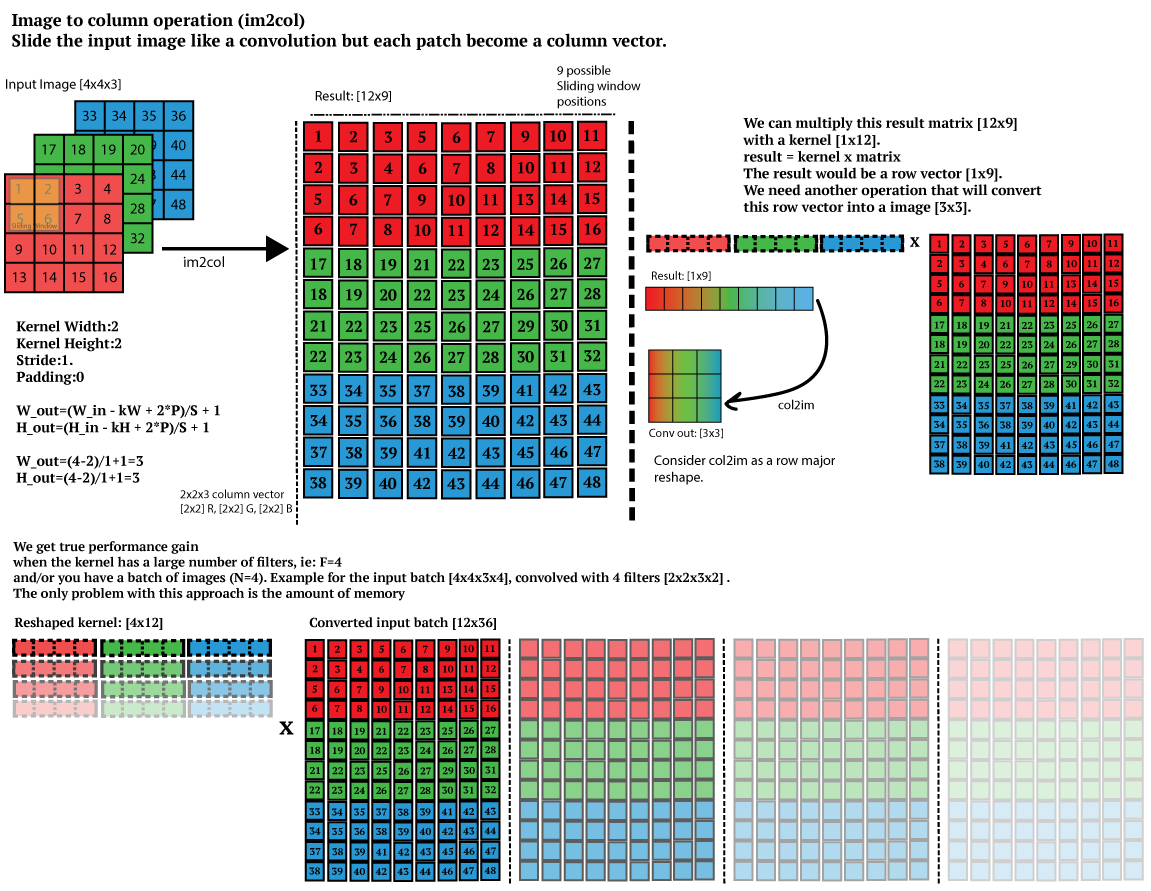
\includegraphics[width=0.85\textwidth]{im2col.png}
\caption{\textsf{im2col} algorithm scheme using a $2\times2$ filter on a image with 3 channels.
At the end of the \textsf{im2col} algorithm the \textsf{GEMM} is performed between weights and input image.
}
\label{fig:im2col}
\end{figure}
\end{center}

Taking into account what we have learned from the DNN models, we can re-formulate our problem using an efficient manipulation of the involved matrices to optimize the \textsf{GEMM} algorithm.
A direct convolution on an image of size ($W\times H\times C$), using a kernel mask of dimensions ($k \times k$), requires $O(WHCk^2)$ operations and thus several matrix products.
We can re-arrange the involved data to optimize this computation and evaluate a single matrix product: this re-arrangement is called \textsf{im2col} (or \textsf{im2row}) algorithm.
The algorithm is just a simple transformation which flats the original input into a bigger matrix, where each column carries all the elements which have to be multiplied for the filter mask into a single step\footnote{
  We work under the assumption that the weights matrix is already a flatten array and thus each row of the weights matrix represents the full mask.
}.
In this way we can immediately apply our \textsf{GEMM} algorithm on the full image.
In Fig.~\ref{fig:im2col} the main scheme of this algorithm is reported.
This algorithm optimizes the computational efficiency of the \textsf{GEMM} product but we have to store a lot of memory for the input re-organization in payback.

Using the mathematical theory behind the problem a third idea can arise using the well known Convolution Theorem: the Fourier transformation of our functions (that in this case are given by the input image and the weights kernel) can be reinterpreted into a simple matrix product in the frequency space.
This is certainly the most \quotes{physical} approach to solve this problem and probably the easier one since the Fourier Transformation is a well-known optimized algorithm, with several efficient implementations provided in literature.
One of the most efficient one is provided by the \textsf{FFTW} (\emph{Fast Fourier Transform in the West}) library~\cite{FFTW05}: \textsf{FFTW3} is an open source \textsf{Ansi-C} subroutine library for computing the Discrete Fourier Transform (DFT) in multiple dimensions, without constraints in input sizes or data types.
The library is not only computationally accurate, but it also provides an efficient parallel version for multi-threading applications.

A further implementation kind is given by linear algebra considerations (very closed to numerical considerations) and it is called \textsf{Coppersmith-Winograd algorithm}.
This algorithm was designed to optimize the matrix product and, in particular, to reduce the computational cost of its operations.
Suppose we have an input image given by just 4 elements and a filter mask with size equal to 3:

\begin{equation}
\mbox{img} = \left[\begin{array}{cccc} d0 & d1 & d2 & d3 \end{array}\right] \quad\quad \mbox{weights} = \left[\begin{array}{ccc} g0 & g1 & g2 \end{array}\right]
\end{equation}
\\
we can now use the \textsf{im2col} algorithm previously described and reshape our input image and weights into

\begin{equation}
\mbox{img} = \left[
\begin{array}{ccc}
d0 & d1 & d2 \\
d1 & d2 & d3
\end{array}
\right],
\quad\quad
\mbox{weights} = \left[
\begin{array}{c}
g0 \\
g1 \\
g2
\end{array}
\right]
\end{equation}
\\
given this data, we can simply compute the output as the matrix product of this two matrices.
The Winograd algorithm rewrites this computation as follow:

\begin{equation}
\mbox{output} = \left[
\begin{array}{ccc}
d0 & d1 & d2 \\
d1 & d2 & d3
\end{array}
\right]
\left[
\begin{array}{c}
g0 \\
g1 \\
g2
\end{array}
\right] = \left[
\begin{array}{c}
m1 + m2 + m3 \\
m2 - m3 - m4
\end{array}
\right]
\end{equation}
\\
where

\begin{equation}
\begin{aligned}
m1 = (d0 - d2)g0\quad\quad m2 = (d1 + d2)\frac{g0 + g1 + g2}{2}
\\
m4 = (d1 - d3)g2\quad\quad m3 = (d2 - d1)\frac{g0 - g1 + g2}{2}
\end{aligned}
\end{equation}
\\
where we can easily notice that the two fractions in $m2$ and $m3$ involve only weight quantities and thus they could be computed only one time for each filter (at each step).
Moreover, we have to manage $4$ \textsf{ADD} and $4$ \textsf{MUL} operations to calculate the $m_i$ quantities and $4$ other ADD to compute the result.
In doing normal matrix products we have to do $6$ \textsf{MUL} operations instead of $4$: the reduction of computational expensive \textsf{MUL} operations by a factor $1.5$x is very significant\footnote{
  A multiplication takes $7$ clock-cycles in a normal CPU while an add takes only $3$ clock-cycles.
}.
In this simple example we use a so-called $F(4, 3)$, i.e image of size $4$ and kernel of size $3$ which gives us $2$ convolutions.
More general formulations are $F(m\times m, r \times r)$ and if we use an image of size $4\times4$ and a kernel of size $3\times3$ we can compare the $16$ \textsf{MUL}s of the \textsf{Winograd} algorithm against the $36$ \textsf{MUL}s which are required by the normal matrix product ($2.25$x).
The \textsf{Winograd} efficiency has been widely proved for CNNs, especially when the kernel size is small.
In our \textsf{Byron} library we provide its implementation for kernel sizes equal to $3$, since the numerical generalization is not straightforward\footnote{
  We would also highlight that this formulation is valid only if we consider unitary strides.
}.

We tested the computational-time of each algorithm on different random images.
The tests were performed on a classical bioinformatics server (128~GB RAM memory and 2 CPU E5-2620, with 8 cores each) and we considered only kernel sizes equal to $3$ (\textsf{Winograd} constrain) varying input dimensions and number of filters.
In Fig.~\ref{fig:winograd_timing} we show the results of our simulations using the \textsf{im2col} values as reference\footnote{
  The \textsf{im2col} algorithm can be found in the major part of Neural Network library and it is also the only convolution function implemented in the \textsf{darknet} library, which is a reference for our work.
}.

\begin{figure}[htbp]
\centering
\def\svgwidth{0.8\textwidth}
\input{./img/winograd_timing.pdf_tex}
\caption{Time performances of different convolution algorithms: \textsf{im2col} (orange, reference), \textsf{FFTW3} (green, fast Fourier transformation using the \textsf{FFTW3} library) and \textsf{Winograd} (blue).
The values are normalized according to the \textsf{im2col} results since it is the most common convolution algorithm.
The tests were performed on different input sizes (width/height), keeping fixed the number of channels and the number of filters.
The tests were performed using a \textsf{C++} implementation of the three methods.
}
\label{fig:winograd_timing}
\end{figure}

In all our simulations we found a visible speedup using the \textsf{Winograd} algorithm against the other two algorithms: for small dimensions we obtained more than $5$x against the \textsf{im2col} and $25$x against the \textsf{fftw} implementation.
The worst algorithm is certainly the \textsf{fftw} one which, despite the efficient \textsf{FFTW3} parallel-library, is always more than $5$ times slower than the reference.
However, it is interesting notice how the \textsf{fftw} implementation is able to reach the best performances when the dimensions are proportional to powers of $2$, as expected from the mathematical theory behind the Discrete Fourier Transformation.

We can conclude that the \textsf{Winograd} algorithm is certainly the best choice when we have to perform a 2D convolution.
The payback of this method is given by the rigid constraints related to the mask sizes and strides: when it is possible it remains the best solution, but in all the other cases the \textsf{im2col} implementation is a relatively good alternative.
The efficiency of \textsf{Byron} library follows the efficiency of the \textsf{Winograd} algorithm, since the major part of layers in modern deep learning Neural Network models are Convolutional layers with sizes equal to $3$ and unitary strides.

%https://victorzhou.com/blog/intro-to-cnns-part-1/


\end{document}

\documentclass{standalone}

\begin{document}

\subsection[Pooling function]{Pooling function}\label{NN:pooling}

Output Neural Network feature maps often suffer of sensitivity on feature location in the input.
One possible approach to overcome this problem is to down sample the feature maps making the resulting feature map more robust to changes in the position.
Pooling functions perform this kind of down sample and they reduce the spatial dimension (but not depth) of the input.
Their use represents an important computational performance improver tool (less feature, less operations) and a useful dimensionality reduction method.
The reduction of feature quantity can also prevent over-fitting problems and it improves the classification performances.

Pooling layers are intrinsically related to Convolutional layers.
The analogy lives in the filter mapping procedure which produces the output in both methods.
While in the Convolutional layer we map a filter over the input signal and we apply a multiplication of the layer weights and the signal values, in the pooling layer we simply change the filter function keeping the same filter mapping procedure (see section~\ref{NN:convolutional} for more informations).
The input parameters of the method are the same of the Convolutional one: the input dimensions, the kernel size and (optional) the stride value.

The most common pooling layers are the Average Pool and the Maximum Pool.
The Average Pool layer performs a down sampling on the batch of images.
It slides a 2D kernel of arbitrary size over the image and the output is the mean value of the pixels inside the kernel.
In Fig.~\ref{fig:avgpool} are shown some results obtained by performing an average pool with different kernel sizes.
Also in this case this test was obtained using our NumPyNet library.

\begin{center}
\begin{figure}[htbp]
\centering
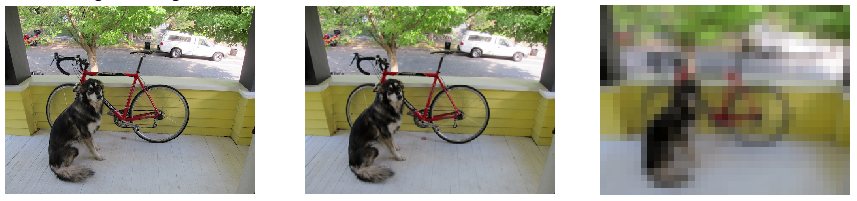
\includegraphics[width=0.85\textwidth]{avgpool_layer.png}
\caption{Average Pool functions applied on a testing image.
\textbf{(left)} The original image.
\textbf{(center)} Average Pool output obtained with a kernel mask $(3\times 3)$.
\textbf{(right)} Average Pool output obtained with a kernel mask $(30\times 30)$.
}
\label{fig:avgpool}
\end{figure}
\end{center}

If in the Convolutional layers a key role was played by the matrix product, in the Pooling layers we have to carefully manage the mapping operations to obtain optimal results.
In particular we would to show the efficient implementation provided into NumPyNet.

In the previous sections we introduced the \textsf{im2col} algorithm which is an efficient method to re-organize the input data.
The same algorithm can also be applied for Pooling layers and thus evaluate the Pooling function (avg, max, etc.) on each row of the re-arranged matrix.
The implementation of the \textsf{im2col} algorithm in Python requires the evaluation of multiple indexes using complex formulas.
Since the NumPyNet library was founded on the Numpy package we can provide an alternative implementation using the \textsf{view} functionality of the library.
A \textsf{view} of a given array is simply another way of viewing its data: technically that means that the data of both objects is shared and thus no copies are created.
In particular we can use the deeper functions of the Numpy package to create a re-organization of our data according to the desired output\footnote{
  The same technique was also used for the implementation of the Convolutional layer in the NumPyNet library.
}.
In the following code we show our implementation of the Average Pooling layer:

\lstset{style=snippet}
\begin{lstlisting}[language=Python, caption=NumPyNet version of AvgPool function, label=code:py_avgpool]
import numpy as np

class Avgpool_layer(object):

  def __init__(self, size=(3, 3), stride=(2, 2)):

    self.size = size
    self.stride = stride
    self.batch, self.w, self.h, self.c = (0, 0, 0, 0)
    self.output, self.delta = (None, None)

  def _asStride(self, input, size, stride):

    batch_stride, s0, s1 = input.strides[:3]
    batch,        w,  h  = input.shape[:3]
    kx, ky     = size
    st1, st2   = stride

    # Shape of the final view
    view_shape = (batch, 1 + (w - kx)//st1, 1 + (h - ky)//st2) + input.shape[3:] + (kx, ky)

    # strides of the final view
    strides = (batch_stride, st1 * s0, st2 * s1) + input.strides[3:] + (s0, s1)

    subs = np.lib.stride_tricks.as_strided(input, view_shape, strides=strides)
    # returns a view with shape = (batch, out_w, out_h, out_c, kx, ky)
    return subs

  def forward(self, input):

    self.batch, self.w, self.h, self.c = input.shape
    kx, ky = self.size
    sx, sy = self.stride

    input = input[:, : (self.w - kx) // sx*sx + kx, : (self.h - ky) // sy*sy + ky, ...]
    # 'view' is the strided input image, shape = (batch, out_w, out_h, out_c, kx, ky)
    view = self._asStride(input, self.size, self.stride)

    # Mean of every sub matrix, computed without considering the pad(np.nan)
    self.output = np.nanmean(view, axis=(4, 5))

\end{lstlisting}

A key role in this implementation is played by the \textsf{\_asStride} function: it returns a view of the original array in which all the masks are organized into a single list.
Using this data re-arrangement we can easily compute the desired pooling function (average in this example) according to the appropriated axes.
We would stress that no copies are produced during this computation and thus we can obtain a faster execution than other possible implementations (e.g \textsf{im2col}).

\end{document}

\documentclass{standalone}

\begin{document}


\section[BatchNorm function]{BatchNorm function}\label{batchnorm}

A common practice before the training of a Neural Network model is to apply some preprocessing to the input patterns.
A classical example is the normalization of training set, i.e it resembles a normal distribution with zero mean and unitary variance.
The initial preprocessing is useful to prevent the early saturation of non-linear activation functions (see section~\ref{activation}).
Moreover in this case we can ensure that all inputs are in the same range of values.

In a deep neural network architecture we can find the same problem also into the intermediate layers because the distribution of the activations is constantly changing during training.
This behavior produces a slowdown in the training convergence because each layer have to adapt itself to a new distribution of data in every training step (or \emph{epoch}).
This problem is also called \emph{internal covariate shift}.

A second problem arises from the heterogeneity of available input data.
If we tune the model parameters according to a given set of data which inevitably be limited we can meet problems during the generalization, i.e the validation of our model using new data, to new samples if they belongs to an equivalent but deformed distribution.
A classical example is given by the image detection: if we train a Neural Network model using gray-scale images we can find generalization problem using colored images.

BatchNorm function (Batch Normalization) allows to overcome these problems with a continuous rescaling of the Neural Network intermediate values during the training\footnote{
  The input data to feed the Neural Network model are commonly packed into a series of \emph{batches}, i.e small subsets of data.
  The BatchNorm function takes its name from this nomenclature and it processes each batch independently.
}~\cite{Sergey2015BatchNorm}.
In particular, the method processes the input of a given layer in order to fight the internal covariate shift problem removing the batch mean and normalizing by the batch variance:

$$
\mu_B = \frac{1}{m}\sum_{i=1}^{m}x_i \quad\quad {\sigma_B}^2 = \frac{1}{m-1}\sum_{i=1}^{m}(x_i - \mu_B)^2
$$
\\
and so the input data becomes:

$$
\hat{x_i} = \frac{x_i - \mu_B}{\sqrt{{\sigma_B}^2 + \epsilon}}
$$
\\
where we add an extra $\epsilon$ in the denominator for numerical stability\footnote{
  The floating point numbers into a computer have finite precision and the variance can underflow bringing to infinite values in the BatchNorm equation.
}.
After this common rescaling we also a apply a scaling-shift to previous results:

$$
y_i = \gamma\hat{x_i} + \beta
$$
\\
where the $\gamma$ and $\beta$ coefficients are left as variables to be tuned during the training (they are learned during training).
The updating rule of the function parameters ($\gamma$ and $\beta$) is given by the simple derivative of the previous function. % maybe insert backprop formulas
In this way we can ensure more stability of the extracted features~\cite{Lecun2000EffBackProp} during the training a faster convergence.

Since the BatchNorm function is became a sort of standard into a deep learning models an efficient implementation of this algorithm is essential to achieve the best computational performances.
We have also to take in count that the batch-normalization procedure is commonly performed after a fully-connected layer or a convolutional one.
Thus the best performances could be obtained merging the two functionality as much as possible as suggested in~\cite{AlexeyAB}.
In the next sections we will show our implementation of the algorithm and we discuss about the code optimization performed\footnote{
  The Byron library was inspired by the \emph{darknet} library provided by Redmon J. et al. and by its many branches.
  Despite in each implementation we can find the BatchNorm function, aware of the author, in any version we can find a right implementation of this function as standalone method.
  We have already highlighted that this normalization function can be efficiently joined to other function to increase the computational performances but in these case we have to different manage the dimensions of the involved arrays.
  A standalone implementation of the BatchNorm function required a rearrangement of its functions and it was provided into the Byron library.
  This was one of the various improvements provided by Byron against the other \emph{darknet}-like libraries.
}.

\end{document}

\documentclass{standalone}

\begin{document}


\section[Shortcut]{Shortcut function}\label{shortcut}


\end{document}

\documentclass{standalone}

\begin{document}


\section[Route]{Route function}\label{route}

\end{document}

\documentclass{standalone}

\begin{document}

% https://medium.com/@hirotoschwert/introduction-to-deep-super-resolution-c052d84ce8cf

\subsection[Pixel Shuffle]{Pixel Shuffle}\label{NN:shuffler}

Pixel Shuffle layer is one of the most recent layer type introduced in modern deep learning Neural Network.
Its application is closely related to the single-image super-resolution (SISR) research, i.e the ensemble techniques which aim at restoring a high-resolution image from a single low-resolution one (see section~\ref{SR:sr} for further details).

The first SISR Neural Networks start with a preprocessing of low-resolution images in input with a bi-cubic up-sampling.
Then the image, with the same dimensions of the desired output, feeds the model which aim to increase the resolution and fix its details.
In this way the amount of parameters and moreover the computation required by the training section increase (by a factor equal to the square of the desired up-sampling scale), despite the required image processing is smaller.
To overcome this problem a Pixel Shuffle transformation, also known as \emph{sub-pixel convolution}, was introduced~\cite{Wenzhe2016Shuffle}: in this work the authors proofed the equivalence between a regular transpose convolution, i.e the previous standard transformation to enlarge the input dimensions, and the sub-pixel convolution transformation without losing any information.
The Pixel Shuffle transformation reorganize the low-resolution image channels to obtain a bigger image with few channels.
An example of this transformation is shown in Fig.~\ref{fig:pixel_shuffle}.

\begin{figure}[htbp]
\centering
\def\svgwidth{0.7\textwidth}
\input{./img/pixel_shuffle.pdf_tex}
\caption{Pixel Shuffle transformation.
On the left the input image with $scale^2$ (:= 9) channels.
On the right the result of Pixel Shuffle transformation.
Since the number of channels is perfect square the output is a single channel image with the rearrangement of the original ones.
}
\label{fig:pixel_shuffle}
\end{figure}

Pixel Shuffle rearranges the elements of the input tensor expressed as $H \times W \times C^2$ to form a $scale \cdot H \times scale \cdot W \times C$ tensor.
This can be very useful after a convolution process, in which the number of filters chosen drastically increase the number of channels, to \quotes{invert} the transformation like a sort of \emph{deconvolution} function.

The main gain in using this transformation is the increment of computational efficiency of the Neural Network model.
The introduction of Pixel Shuffle transformation in the Neural Network tail, i.e after a sequence of small processing steps which increase the number of features, reorganize the set of features into a single bigger image, i.e the desired output in a SISR application.
The feature processing steps, which generally are faced on with convolutional layers, can be performed with smaller images in input and thus can be obtained faster since the up-scaling task will be performed by a single Pixel Shuffle transformation.

Despite this transformation has became a standard in super-resolution applications and thus it can be found into the most common deep learning libraries (e.g \emph{Pytorch} and \emph{Tensorflow}) a C++ implementation is hard to find.
Moreover, each library implements the transformation following its own data organization\footnote{
  The main difference between \emph{Pytorch} and \emph{Tensorflow} is related to the storage organization of the image.
  \emph{Tensorflow} has a \quotes{standard} input assessment as $H \times W \times C$.
  \emph{Pytorch} has a so-called channel-first implementation and so the input tensor is organized as $C \times H \times W$.
}.
For this reason we proposed in our libraries a dynamic version of the algorithm in C++ able to perform both versions of the algorithm.

The algorithmic implementation of the pixel-shuffle transformation is essentially a re-indexing of the input values.
While in a C++ implementation of the algorithm we could obtain the desired result inside a sequence of nested for loops playing with the loop indexes, for an efficient Python version we used a sequence of transposition and reshaping to rearrange the input values.
The following snippet shows the NumPyNet version of this algorithm.

\lstset{style=snippet}
\begin{lstlisting}[language=Python, caption=NumPyNet version of Pixel-Shuffle function, label=code:py_shuffle]
import numpy as np

class Shuffler_layer(object):

  def __init__(self, scale):

    self.scale = scale
    self.scale_step = scale * scale

    self.batch, self.w, self.h, self.c = (0, 0, 0, 0)

    self.output, self.delta = (None, None)

  def _phase_shift(self, input, scale):
    b, w, h, c = input.shape
    X = input.transpose(1, 2, 3, 0).reshape(w, h, scale, scale, b)
    X = np.concatenate(X, axis=1)
    X = np.concatenate(X, axis=1)
    X = X.transpose(2, 0, 1)
    return np.reshape(X, (b, w * scale, h * scale, 1))

  def _reverse(self, delta, scale):
    # This function apply numpy.split as a reverse function to numpy.concatenate
    # along the same axis also

    delta = delta.transpose(1, 2, 0)

    delta = np.asarray(np.split(delta, self.h, axis=1))
    delta = np.asarray(np.split(delta, self.w, axis=1))
    delta = delta.reshape(self.w, self.h, scale * scale, self.batch)

    # It returns an output of the correct shape (batch, in_w, in_h, scale**2)
    # for the concatenate in the backward function
    return delta.transpose(3, 0, 1, 2)

  def forward(self, input):

    self.batch, self.w, self.h, self.c = input.shape

    channel_output = self.c // self.scale_step # out_c

    # The function phase shift receives only in_c // out_c channels at a time
    # the concatenate stitches together every output of the function.

    self.output = np.concatenate([self._phase_shift(input[:, :, :, range(i, self.c, channel_output)], self.scale)
                                  for i in range(channel_output)], axis=3)

    self.delta = np.zeros(shape=self.out_shape, dtype=float)

  def backward(self, delta):

    channel_out = self.c // self.scale_step # out_c

    # I apply the reverse function only for a single channel
    X = np.concatenate([self._reverse(self.delta[:, :, :, i], self.scale)
                                      for i in range(channel_out)], axis=3)


    # The 'reverse' concatenate actually put the correct channels together but in a
    # weird order, so this part sorts the 'layers' correctly
    idx = sum([list(range(i, self.c, channel_out)) for i in range(channel_out)], [])
    idx = np.argsort(idx)

    delta[:] = X[:, :, :, idx]

\end{lstlisting}

The two functions \textsf{\_phase\_shift} and \textsf{\_reverse}\footnote{
  These function are \quotes{private} function of the object class.
}
produce the re-arrangement of the indexes according to the pixel-shuffle transformation and its inversion\footnote{
  During the back-propagation, in fact, we have to apply the reverse transformation to the gradient.
}
In the forward function we apply the \textsf{\_phase\_shift} to the sequence of channels (in the right order) and then we concatenate the results into a single tensor (output).
The backward function instead needs a re-ordering of channel sequence after the concatenation.

As told above, in the C++ implementation provided into the Byron library we can compute the desired re-indexing using a series of nested for loops.
An equivalent solution can be obtained also by the contraction of the loops into a single one using divisions to obtain the right indexes.
This solution was taken in count into the first version of the library but the amount of required divisions weights on the computational performances.
The division operations are the most computationally expensive operations in terms of CPU clock-time.
The old versions of OpenMP multi-threading library forced the users to spend time in the evaluation of the \quotes{loop-contraction} to obtain the better performances by a single parallel for loop.
The new features of OpenMP library provide the very powerful \emph{collapse} keyword which performs an automatic loop-contraction.
The keyword can be applied only with a series of independent and perfectly nested\footnote{
  Two for loops are perfectly nested if there are not other code lines between them.
}
for loops which is exactly our case.
Moreover we have not to take in care any thread concurrency trouble since the iterations, as the output indexes, are totally independent.
We widely used the \textsf{collapse} keyword in the Byron library to simplify the code and the function evaluation but the Pixel-Shuffle case is one of the most efficient one, since we could collapse six nested loops\footnote{
  In the Pixel-Shuffle we have to loop over batch, width, height, channels plus a couple of loops over the scale factor that we want to apply.
  In total we have to manage six dimensions that can be easily collapsed into a single one given by their product.
} (ref. \href{https://github.com/Nico-Curti/Byron/blob/master/src/shuffler_layer.cpp}{on-line}.

\end{document}

\documentclass{standalone}

\begin{document}

\subsection[Cost function]{Cost function}\label{NN:cost}

A machine learning algorithm is used to minimize or maximize a cost function.
In other words when we implement a machine learning algorithm we want to know how good is our result according to prior knowledge about the desired results.
So we have to establish a function ables to represent the error of our model.
This kind of function are commonly called \emph{error functions} or \emph{loss functions} or just simply \emph{cost function}.
In the previous sections we have shown many algorithms used into a Neural Network model and we have talked about how to update the functional parameters according to the evaluated error.
This error is provided by the cost function.

The cost function represents the final output of our Neural Network model so it is reasonable to talk about it at the end of this chapter.
There are many kinds of loss functions and there is not a particular one able to works with all kinds of data.
So we have to pay attention to chose the right one in our problems.
In particular we have to take in count the possible presence of outliers, the structure of our model, the computational efficiency of our algorithm and most of all the number of classes that we want to predict.
Broadly, we can classify the loss functions into two major categories: the classification losses and the regression losses.
In the first case we want to predict a finite number of categorical values (classes).
In the second case the prediction is performed on a series of continuous values.
Since in this work we are focusing only on classification problems we will only talk about the first case.

The most common cost function is given by the \emph{Mean Square Error} (MSE) or \emph{L2 loss} (very closed to the regularization function hinted at the end of \ref{NN:batchnorm}).
Its mathematical formulation is quite simple and it is given by

$$
MSE = \frac{\sum_{i=1}^{N}\left( y - t \right)^2}{N}
$$
\\
where we follow the nomenclature given in \ref{NN:perceptron} and $N$ is the number of output which is equivalent to the number of classes.
It is one of the most used cost function due to its simplicity either from a mathematical either from a numerical point of view.
The possible range of values ranged from 0 to $\infty$.
With MSE function the predictions which are far away from actual values are heavily penalized, due to the squaring.

A slight different function is given by the \emph{Mean Absolute Error} (MAE) or \emph{L1 loss} in which we replace the squaring with a module of the error.

$$
MAE = \frac{\sum_{i=1}^{N}|\left( y - t \right)|}{N}
$$

With MAE we loose the information about the error direction (preserved by the squaring in MSE) and just simply evaluate the absolute value of it.

The main differences between these two functions can be summarized as follow: using the MSE function we can easily solve the problem but the MAE function is more robust against possible outliers.
Despite both functions reach the minimum in a perfect classification configuration (error equal to zero), in presence of outliers we have to manage with large differences in the numerator of the function.
With large differences, the square values are greater than the absolute values but while the MSE tries to adjust its performance to minimize those cases, the other samples pay the higher cost.

A problem related to the MAE function arises during the gradient evaluation.
Its gradient, in fact, is the same throughout, which means that we will have large gradient values also with small differences which is a worse configuration during the training.
A simple possible workaround is to introduce a shrinking parameter, given by a dynamic learning rate, when we move closer to the minimum.

When we have to manage multi-class problems there are other common cost functions based on likelihood scores.
The simpler one is the \emph{Cross Entropy loss} or \emph{Log loss}:

$$
CrossEntropyLoss = -(y\cdot\log(t) + (1 - y)\cdot\log(1 - t))
$$

This function just multiply the log of the actual predicted probability by the ground truth class.
In this way when we have two classes (e.g $t \in [0, 1]$) we can alternatively nullify the two parts of the function\footnote{
  When the actual label is equal to 1, i.e $y=1$, the second half of the Log Loss function disappears whereas in case of actual label is equal to 0 the first half is null.
}.
In this way the loss function heavily penalizes the predictions that are confident but wrong.
This function works with binary classification problems where the output classes are binned in $[0, 1]$.
For this reason the output of the model must be constrained into the $[0, 1]$ domain and thus a proper activation function should be provided.
Classically this loss function is used jointly to the sigmoid activation (ref.~\ref{NN:activation}) which constrains the output of the model in the desired interval.
For this reason in our implementation of the algorithm we chose to merge the sigmoid function and the Log Loss function into a single object\footnote{
  We also try to prevent wrong uses of this loss function for laypersons.
  This implementation was already suggested by the \emph{darknet} library so we simply propagate it in our implementations.
}.

A last duty to mention loss function is the extension of the Log loss to multiple classes, the so-called \emph{Categorical Cross Entropy Loss}.

$$
CategoricalCrossEntropyLoss = -\sum{i=1}^{N}\left( y\cdot\log(t) \right)
$$

This function generalized the previous one for multiple-classes, i.e for problems where the correct output can be only one.
The loss compare the distribution of the predictions, i.e output of the model, with the prior known distribution.
In this way only the probability of the true class will be 1 and all the other classes will be set to 0.
Also in this case we have to pay attention to the output of our model which is intended as a probability value ranging in $[0, 1]$.
In particular this function commonly works jointly to a softmax activation function.
As in the previous case we chose to implements this loss function in a separated object associated to the softmax transformation.

Many other loss function can be mentioned to overcome different kind of problems.
The list of presented loss function was related to the implementation of the \emph{darknet}-like library which are ported also into the NumPyNet and Byron libraries, i.e either in Python and C++.
NumPyNet and Byron libraries also provided a wider list of loss functions to improve the usability of them and improve their computation (and fixed some \emph{darknet} issues).
A full list of available loss functions can be found in the \href{https://github.com/Nico-Curti/Byron/blob/master/src/cost_layer.cpp}{on-line} version of the libraries with a list of easily visual examples.

A further improvements was given from a numerical point-of-view: many mathematical formulas needs expensive math operations as logarithms and trigonometric functions.
An efficient (but approximated) math formulas was implemented both in the C++ and Python to reach faster computational performances.
These numerical math operations are widely used into the Byron library to increase the performances despite their used can be turned off by user at compile time in Byron.
The full set of functions, in fact, is enclosed into a \textsf{macro} definition (\textsf{\_\_fmath\_\_}) that can be enabled at compile-time.

A classical example of this faster math operation is given by the \emph{fast inverse square root} algorithm, firstly introduced in 1999 in the source code of \emph{Quake III Arena}, a first-person shooter video game.
The method is based on a Newton algorithm which can be stopped at the desired precision order: less precision is associated to faster execution, obviously.
In our \textsf{fast math} implementation we provide a set of Newton algorithms associated to the most common mathematical operations, like \textsf{exp}, \textsf{log}, \textsf{sqrt} and so on.
We tested these implementations against the common standards (Numpy package for Python and \textsf{std::} for C++) and we compare the time execution performances (we required a precision of at least $10^-4$).
The obtained results are shown in Fig.~\ref{fig:fmath} where we normalized the execution time taking Numpy implementation as reference.

\begin{figure}[htbp]
\centering
\def\svgwidth{0.8\textwidth}
\input{./img/fmath_timing.pdf_tex}
\caption{Time performances of standard mathematical operations implemented through Newton approximations.
We compare the results obtained with the Numpy library (blue, reference) and the standard C++ library (\textsf{CMath}) to their equivalent into the custom \textsf{FMath} version.
In the comparison we have to take in mind that the Numpy library is based on a C++ wrap and that the Python version of the \textsf{FMath} is written in pure Python language.
In all the cases the \textsf{FMath} version of the functions performs better or at-least-equal to the standard one.
}
\label{fig:fmath}
\end{figure}

As can be see all the results obtained by the \textsf{fast math} algorithms are faster or at least equals to the standard ones.
The C++ version of the \textsf{fast math} is certainly the better choice for an efficient implementation of the algorithms in all the cases and it is interesting to notice how some functions (\textsf{pow2} and \textsf{log10}) are drastically slower in C++ than in Python, despite the intrinsic overhead of the Python language.
This is probably due to particularly optimizations performed by the Numpy package in the implementation of these special cases: if we compare those functions to the general ones (\textsf{pow} and \textsf{log}), in fact, the results confirm the efficiency of the C++ language.

These results highlight the importance of code testing before release it: we have to pay always attention in writing a code and query also the standard choices.


\end{document}


\documentclass{standalone}

\begin{document}

\section[Object Detection]{Object Detection}\label{obj_detection:obj}

Object detection is one of the larger deep learning sub-discipline, especially when we talk about Neural Network models.
This kind of problems aim to identify single or multiple objects into a picture or video stream.
The possible applications of these tools are everywhere these days and they involve object tracking, video surveillance, pedestrian detection, anomaly detection, people counting, self-driving cars or face detection and the list goes on.

There are many machine learning and deep learning techniques proposed during the years about this topic and each one has its own pros and cons.
The most prominent and moder techniques involve the use of very deep Neural Network models, with a huge amount of parameters to tune.
The most famous ones are probably the Faster R-CNN (\emph{Faster Region Convolutional Neural Network})~\cite{ren2015faster} and its \quotes{evolution} into the YOLO (\emph{You Only Look Once}) model~\cite{redmon2015look, redmon2016yolo9000, redmon2018yolov3}.

The R-CNN models are one of the state-of-art CNN-based deep learning object detection model and their evolution into Fast R-CNN tries to improve their speed.
The standard approach for object detection is based on moving a \emph{sliding window} to search in every position of the image the objects.
However, the intrinsic problems of these kinds of methods are the window dimensions and the large computation required to map with multiple window sizes the full image.
Different objects, or even the same kind of objects, could have different aspect ratios and sizes in relation to the position of the camera which captured the image or to their distances.
R-CNN models try to overcome these problems generating about \numprint{2000} region proposals, i.e bounding boxes, and applying to each one a image classification procedure, using a standard CNN.
Finally, each detected region can be refined using a regression approach.

A Faster R-CNN model is based on the same idea but, instead of feeding the bounding boxes to the CNN, it feeds the input image to the CNN to generate a convolutional feature map.
Starting from this feature map we can easier identify the region of proposals (Region Proposal Network) and warp them into squares.
The list of these regions are then reshaped using a Polling layer and processed by a fully connected layer.
The advantages of Faster R-CNN are thus visible: we do not need to feed \numprint{2000} region proposals to the CNN every time, but the feature map is generate once per image using the convolution operation.
In this way we can also separate the feature map creation to the selective search algorithm.

A key role on these models is given by the \emph{anchor} concept: an \emph{anchor} is essentially a box and it identifies the shape of a portion of the input image at different scale levels.
The CNN feature map feeds the Region Proposals Network which uses a sliding window over it, generating $k$ anchor boxes.
These boxes are certainly fewer than the previous cited \numprint{2000} windows.

A breakthrough idea on the real-time object detection was the introduction of the YOLO model.
The model was developed by Redmon et al. at Washington University and it is probably the state-of-art on object detection, especially for its very incredible speed (it can reach 45 FPS on modern GPUs!).
Certainly it is the faster method publicly available, but its popularity is also due to its innovative strategy in object detection.
Despite all the other algorithms use regions to localize the object into the image, the YOLO network does not look at the complete image but only on a parts of it, which has the higher probability to contain an object.
In YOLO a single CNN predicts the bounding boxes and the class probabilities of them.
YOLO slits a single image into a $S\times S$ grid and on each grid $m$ bounding boxes are taken.
For each of them, the CNN outputs a class probability and offset values.
Finally, these bounding boxes are filtered according to their probability and a chosen threshold.

One of the most bigger limitation of this model is that it struggles with small objects.
This is due to the spatial constraints of the algorithm.
Fortunately, in the previous sections we have already discussed on how we can overcome this kind of problem using Super Resolution.
In the next section we will discuss about further characteristics of the YOLO model and about its implementation into the \textsf{Byron} library, considering its efficiency against the original implementation.
Finally, we will join the efficiency of the previous Super Resolution models to the performances of our optimized implementation of YOLO.


%Introduction on the image classification and detection with Yolo architecture.
%Implementation in Byron with description of performances against darknet (original implementation).
%Focus on performances (time, memory, cpu).


\end{document}


\documentclass{standalone}

\begin{document}

\section[Super Resolution]{Super Resolution}\label{SR:sr}

\begin{figure}[htbp]
\def\svgwidth{0.5\textwidth}
\input{./img/sr_wow.pdf_tex}
\quad
\def\svgwidth{0.465\textwidth}
\input{./img/sr_wow2.pdf_tex}
\caption{Single Image Super Resolution.
Between the red lines the super resolved version of the original image.
}
\label{fig:sr_wow}
\end{figure}

The Super Resolution (SR) is a slight novel technique based on Neural Network models which aims to improve the spatial resolution of a given image\footnote{
  The best-known \quotes{implementation} of Super Resolution concerns the microscopy super-resolution.
  In this work we are focusing on algorithms and numerical implementations so we will talk about the numerical counterpart of this technique, totally ignoring the original \quotes{hardware} version.
}.

The first SR methods on digital images estimate the high frequency information of the images, starting from a series of low-resolution (LR) patches and their high-resolution (HR) counterparts.
These patches (ROIs of the LR image commonly smaller than $50\times50$) were extracted after an edge enhancement procedure or a simple 2D Fourier transformation, which extracts the high frequency information.
Collecting these patches an \quotes{association dictionary} between LR and HR was created.
This dictionary was used to learn the correct associations between LR and HR and then applied on new images.
The images considered were of the same dimensions in these firstly applications, i.e the purpose was only to improve the spatial resolution of the image without changing the sampling step.

The idea of use neural network models and in particular convolution functions to face this problem was born in 2014 at the Engineering University of Honk Kong, due to the large popularity of these models during those years.
The increasing computational power allowed to create automatic models able to learn the LR-HR associations without any dictionary.
In this year the SRCNN model~\cite{SRCNN} arises, a three-layer neural network able to learn a large ensemble of features to reproduce the desired associations.
The first layer aimed to extract the LR patches from the input image; the second layer produces the association between the LR patches and the tuned HR ones; the last layer reorganized the HR patches ensemble produced into a single HR image, i.e the output.

From this starting implementation many improvements was performed in this research field, but the fundamental idea is not changed.
Modern models simply have a greater number of layers, due to the increasing computational power availability, and they use appropriated workaround to overcome the (large-)parameters tuning problem.

In the next sections we will show the super resolution technique step-by-step starting from the image pre-processing up to the most modern algorithmic solutions.
At the end of this chapter the \textsf{NumPyNet} and \textsf{Byron} implementations of some modern models will be presented and applied over biomedical images.

%Introduction on Super Resolution problem with focus on state-of-art neural network architecture.
%Description of the Byron implementation and application on NMR data with the most common measurements.
%Super-resolution allows better detection!


\end{document}

\documentclass{standalone}

\begin{document}

\subsection[Resampling]{Resampling}\label{SR:downsampling}

Up to now we have talked about neural network models as classification algorithms.
In the SR problem we have no classes but the desired output is a image.
This behavior is often hard to digest but it does not change anything about the previous consideration.
The only change will be related to the size of the neural network and its amount of parameters that could drastically increase due to the larger output required.
Lets start from the beginning: to feed a super-resolution model we have to use a series of prior-known LR-HR image association.
In the real life we always have a series of images, typically LR images, and we want to enlarge the resolution of them, i.e enlarge the spatial dimensions of the input image, to better see some particulars or just to create an output without artifacts or evident pixel grains.
If we consider these series of images as the HR one we can easily down-sample them without particular troubles\footnote{
  Ignoring particular cases the hardest step is always to enlarge the image resolution and not the inverse step.
}.
This re-sampling will introduce a aliasing factor that our model should learn to nullify.
The number of model parameters is typically around the $10^7$ so if we introduce any filtering process (degradation) in the input image the model will be able to overcome also these problems.

Starting from these considerations we can down-sample our images by a desired scale factor: common scale factor are between 2 and 8 and in this work we will refer to a scaling equal to 4.
A crucial role is played by the re-sampling (or down-sampling) algorithm chosen for the artificial image degradation.
Any down-sampling algorithm, in fact, loose part of the original information by definition.
Thus we can facilitate the learning choosing a lossless one but in this way we will loose in generalization (the model will not learn how to overcome some cases), or we can apply a drastic down-sample technique and achieve better performances later.

The simpler down-sampling algorithm is given by a \emph{nearest interpolation}.
This algorithm pass a kernel mask over the image and it substitutes each pixel mask to their average\footnote{
  The inverse (up-sampling) interpolation simply replicates each pixel in each dimension by a number equal to the scale factor.
}.
This procedure can be achieved using a \emph{Pooling} algorithm (in particular an AveragePooling) (ref.~\ref{NN:pooling} for further informations) for the down-sample or we can use an UpSample layer.
The UpSample function is commonly related to GAN (Generative Adversarial Networks) models in which we have to provide a series of artificial images to a given Neural Network but it is a function which can be introduce inside a Neural Network model to rescale the number of features.
We mention it in this section since it is not intrinsically related to a Neural Network model but it could be use as image processing technique.

We provide an implementation of this algorithm either in \textsf{NumPyNet} either in \textsf{Byron} library using different techniques.
The UpSample function inside a Neural Network model has to provide both up- and down- sampling technique since one is used in the forward function and its inverse during the back-propagation.
To achieve this function in \textsf{NumPyNet} we can use a series of reshapes and striding on the input matrix as shown in the following snippet.

\lstset{style=snippet}
\begin{lstlisting}[language=Python, caption=NumPyNet version of Upsampling function, label=code:py_upsample]
import numpy as np
from numpy.lib.stride_tricks import as_strided

class Upsample_layer(object):

  def __init__(self, stride=(2, 2), scale=1., **kwargs):

    self.scale = float(scale)
    self.stride = stride

    if not hasattr(self.stride, '__iter__'):
      self.stride = (int(stride), int(stride))

    assert len(self.stride) == 2

    if self.stride[0] < 0 and self.stride[1] < 0: # downsample
      self.stride = (-self.stride[0], -self.stride[1])
      self.reverse = True

    elif self.stride[0] > 0 and self.stride[1] > 0: # upsample
      self.reverse = False

    else:
      raise NotImplementedError('Mixture upsample/downsample are not yet implemented')

    self.output, self.delta = (None, None)

  def _downsample (self, input):
    batch, w, h, c = input.shape
    scale_w = w // self.stride[0]
    scale_h = h // self.stride[1]

    return input.reshape(batch, scale_w, self.stride[0], scale_h, self.stride[1], c).mean(axis=(2, 4))

  def _upsample (self, input):
    batch, w,  h,  c  = input.shape     # number of rows/columns
    b,     ws, hs, cs = input.strides   # row/column strides

    x = as_strided(input, (batch, w, self.stride[0], h, self.stride[1], c), (b, ws, 0, hs, 0, cs)) # view a as larger 4D array
    return x.reshape(batch, w * self.stride[0], h * self.stride[1], c)                                     # create new 2D array

  def forward(self, input):
    self.batch, self.w, self.h, self.c = input.shape

    if self.reverse: # Downsample
      self.output = self._downsample(input) * self.scale

    else:            # Upsample
      self.output = self._upsample(input) * self.scale

    self.delta = np.zeros(shape=input.shape, dtype=float)

  def backward(self, delta):
    if self.reverse: # Upsample
      delta[:] = self._upsample(self.delta) * (1. / self.scale)

    else:            # Downsample
      delta[:] = self._downsample(self.delta) * (1. / self.scale)


\end{lstlisting}

Thus the down-sampling algorithm is obtained reshaping the input array according the two scale factors (\textsf{strides} in the code) along the two dimensions and computing the mean along these axes.
Instead the up-sample function use the stride functionality of the \textsf{Numpy} array to rearrange and replicate the value of each pixel in a mask of size \textsf{strides}$\times$\textsf{strides}.

The same functionality can be obtained in the \textsf{C++} version of the code provided by the \textsf{Byron} library in which we compute the right indexes along a nested sequence of for loops (ref. \href{https://github.com/Nico-Curti/Byron/blob/master/src/upsample_layer.cpp}{on-line}).
We have to take in care the summation reduction provided by the down-sampling according to the thread concurrency: in this case we can not generalize the loop collapsing to the full set of lops but we have to separately manage the summation in a sequential section.

A more sophisticated interpolation algorithm, which reduce the loosing informations, is provided by the \emph{bicubic interpolation}.
The re-sampling algorithm interpolate the information provided by the nearest pixels using a cubic function.
Given a pixel, the interpolation function evaluates the 4 pixels around it applying a filter given by the equation:

$$
k(x) = \frac{1}{6} \left\{ \begin{array}{rc}
  (12 - 9B - 6C) |x|^3 + (-18 + 12B + 6C) |x|^2 + (6 - 2B)           & \mbox{if}        |x| < 1 \\
  (−B − 6C) |x|^3 + (6B + 30C) |x|^2 + (−12B − 48C) |x| + (8B + 24C) & \mbox{if} 1 \leq |x| < 2 \\
  0                                                                  & otherwise                \\
  \end{array}
  \right.
$$
\\
where $x$ identify each pixel below the filter.
Commonly values used for the filter parameters are $B=0$ and $C=0.75$ (used by \textsf{OpenCV} library) or $B=0$ and $C=0.5$ used by \textsf{Matlab}\footnote{
  In this case the filter is also called Catmull-Rom filter.
}.
Despite this function was also implemented in the most common library in \textsf{Python} we provide an efficient multi-threading implementation in the \textsf{Byron} library.

Equivalent performances could be achieved using a generalized version of the bicubic filter which use the 8 positions mask around each pixel, the so called Lanczos filter.
Also this function was provided into the \textsf{Byron} library.

To better understand the told above functions we can consider their application on the simple image given in Fig.\ref{fig:resampling}.

\begin{figure}[htbp]
\centering
\def\svgwidth{\textwidth}
\input{./img/up_down_sampling.pdf_tex}
\caption{Re-sampling image example.
\textbf{(left)} The original image.
\textbf{(up right)} The down-sampled blue-ROIs using different interpolation algorithm (Nearest, Bicubic and Lanczos, respectively).
We use a scale factor equal to 2 (half size in down-sampling and double size in up-sampling).
The Lanczos interpolation is the lossless algorithm but from a qualitative point-of-view the result is the quite the same of the bicubic one.
\textbf{(down right)} The up-sampled red-ROIs using the same interpolation algorithm of the upper row.
Also in the Up-sampling the Lanczos and bicubic algorithms produces equal qualitative results.
The Nearest algorithm produces the worse results in both up- down- cases.
}
\label{fig:resampling}
\end{figure}

In the figure the three algorithms were applied over the same image to highlight the differences against the down-sampling and up-sampling.
The nearest interpolation algorithm produces always the worse results both in up-sampling and down-sampling.
In the bicubic and Lanczos down-sampling we can better appreciate the \quotes{preservation} of the line shapes that are lost using the Nearest algorithm.
The result obtained by bicubic and Lanczos are quite similar in both cases but the computational cost of the Lanczos algorithm is greater than the bicubic one.
This is the reason why the bicubic interpolation is the most used technique for image resizing with a balance between computational cost and qualitative results.
In our implementation of SR algorithms we chose to use the bicubic interpolation for those reasons.

The aim of SR algorithm is to overcome these results and obtain a better quality image either from an optical point-of-view either from a mathematical one.
Until now we are considering the quality of the digital image only from a qualitative point-of-view.
In the next section we will introduce some useful mathematical scoring to numerically evaluate the image quality.

\end{document}

\documentclass{standalone}

\begin{document}

\section[Image Quality]{Image Quality}\label{SR:quality}

The most common image quality evaluator is given by our eyes.
This is true also for SR problems: the final purpose still remain to obtain images that are better visible for human eyes, the so called \emph{visual loss}.
We can however provide some mathematical formulas which allows to quantitative evaluate the image quality.
In both cases we need to establish a relation between the original image and the produced one.
Thus we can formulate a quality score only with a reference image.
In SR problems, or more in general in up-sampling problems, we can compare the original HR image with the image obtained by the output of our model.
In this way our quality score will be a measure of similarity between the two images.

The simple similarity score can be obtained evaluating the peak-signal-to-noise-ratio (PSNR).
This quantity is commonly used to establish the compression lossless of an image and it can be computed as

$$
PSNR = 20 \cdot \log_{10}\left( \frac{\max(I)}{\sqrt(MSE)} \right)
$$
\\
where $\max(I)$ is the maximum value which can be taken by a pixel in the image (in general it will be 1 or 255 depending on the image format chosen) and $MSE$ is the Mean Square Error (ref.~\ref{NN:cost}) between the original image and the reconstructed one.
The MSE for an image can be computed as:

$$
MSE = \frac{1}{WH} \sum_{i=1}^{W}\sum_{j=1}^{H} \left( I(i, j) - K(i, j) \right)^2
$$
\\
where $W$, $H$ are width and height of the two images and $I$, $K$ are the original and reconstructed images, respectively.

In other words the PSNR is the maximum power of the signal over the background noise.
It is expressed in decibel (dB) because the image values ranging in a wide interval and the logarithmic function rearrange the domain.
Thus we can conclude that high PSNR values are associated to a good reconstruction of the original image.

The PSNR is probably the most common quality score~\cite{psnr_ssim} but it does not always related to a qualitative visual quality.
Despite it is commonly used as loss function for SR models.

\begin{table}[htbp]
\centering
\begin{tabular}{lccc}
\hline \rowcolor{darkgrayrow}
         & Nearest       & Bicubic        & Lanczos  \\
\hline
PSNR     & 25.118        & 27.254         & 26.566   \\
SSIM     &  0.847        &  0.894         &  0.871   \\
\hline
\end{tabular}
\caption{Image quality scores: PSNR (peak-signal-to-noise-ratio) and SSIM (Structural SIMilarity index).
The values are computed on the image shown in Fig.~\ref{fig:resampling}.
The original image was down-sampled using a Lanczos algorithm and then re-up-sampled using three different algorithms: nearest, bicubic and Lanczos interpolations.
For each interpolation algorithm the PSNR and SSIM was evaluated.
As expected the highest scores were obtained using the bicubic algorithm while the worst reconstruction is performed by the nearest algorithm.
}
\label{tab:psnr}
\end{table}

Considering the series of images shown in Fig.~\ref{fig:resampling} we can evaluate the PSNR score starting from a down-sampled image.
Taking the down-sampled image obtained with the Lanczos algorithm we can compare the original image with their up-sampled version given by the three methods (ref. Tab.~\ref{tab:psnr}).
As expected, the lowest PSNR value is achieved by the nearest interpolation method while the best performances are obtained by the bicubic algorithm.
This confirm the wider use of bicubic method in image processing applications.
Moreover we have to take in account that an increment of 0.25 in PSNR value correspond to a visible improvement for human eyes.

A more advanced quality score, commonly used in super resolution image evaluation, is given by the \emph{Structural SIMilarity index} (SSIM).
The SSIM aims to mathematically evaluate the structural similarity between two images taking into account also the visible improvement seen by human eyes.
The SSIM function can be expressed as

$$
SSIM(I, K) = \frac{1}{N}\sum_{i=1}^{N} SSIM(x_{i}, y_{i})
$$
\\
where $N$ is the number of arbitrary patches which divide the image\footnote{
  Patch dimensions commonly used are $11\times11$ or $8\times8$.
}
For each patch the SSIM is computed as

$$
SSIM(x, y) = \frac{(2\mu_x\mu_y + c_1)(2\sigma_{xy} + c_2)}{ ({\mu_x}^2 + {\mu_y}^2 + c_1)({\sigma_x}^2 + {\sigma_y}^2 + c_2) }
$$
\\
where $\mu$ and $\sigma$ are the means and variances of the images, respectively, and $\sigma_{xy}$ represents the covariance.
The $c_1$ and $c_2$ parameters are fixed to avoid mathematical divergence.
Also in this case higher value of SSIM corresponds to high similarity between the original image and the reconstructed one.

Based on the previous equation we can highlight a link with the pooling functions discussed in~\ref{NN:pooling}.
Also in this case, in fact, we works with a window/kernel moved along the image which applies a mathematical function on the underlying pixels.
This equivalence suggests an easy implementation of this method with slight modifications of the previous code.

The evaluation of SSIM quality score on the previous up-sampled images (ref. Fig.~\ref{fig:resampling} and Tab.~\ref{tab:psnr}) confirms the results obtained by the PSNR.
Also in this case the worst reconstruction is obtained by the nearest algorithm while the highest SSIM is obtained by the bicubic algorithm.
The gap between SSIM values is smaller than PSNR ones but this is due to the different domains of the two functions.

\end{document}

\documentclass{standalone}

\begin{document}

\subsection[Super Resolution Models]{Super Resolution Models}\label{SR:wdsr}

\begin{center}
\begin{figure}[htbp]
\centering
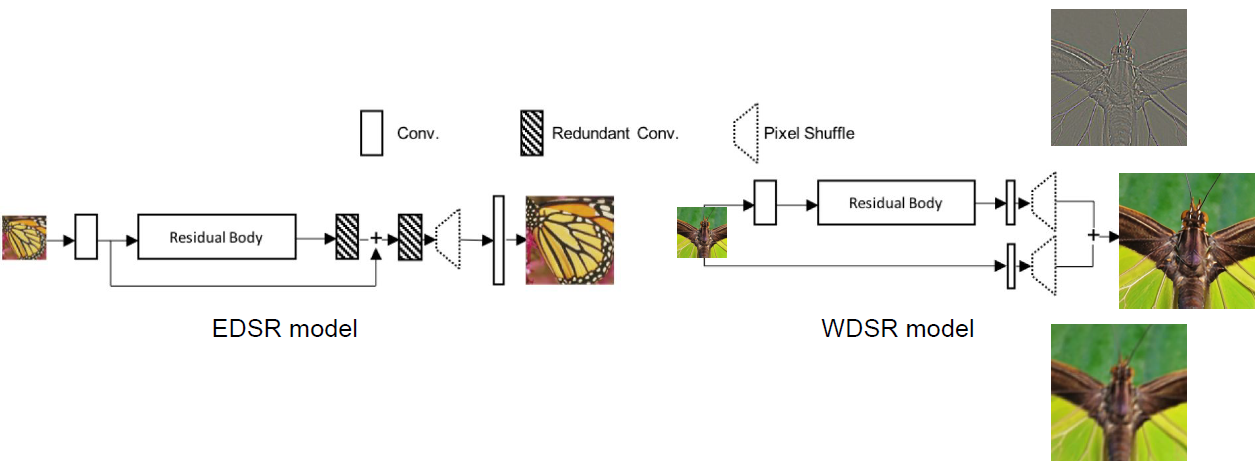
\includegraphics[width=0.85\textwidth]{SR_models.png}
\caption{Super Resolution models analyzed in this word.
\textbf{(left)} EDSR model.
The model is a modified version of the ResNet architecture designed for SISR applications.
The architecture is made by a sequential CNN framework which processes the input image.
The EDSR has more than 43 million of parameters in total.
\textbf{(right)} WDSR model.
The model is the updated version of the EDSR one.
The model optimizes its numerical efficiency using a different approach in the analysis of low- and high-frequency components in the input image.
the WDSR has slight more than 3.5 million of parameters, less than 10\% of the EDSR model.
}
\label{fig:sr_models}
\end{figure}
\end{center}

There were different kind of models proposed for image Super Resolution purposes but in this work we focused only on two of them.
Both are based on deep learning Neural Network models and they became famous in the research community since they both won the last NTIRE editions, 2017 and 2018 respectively.

\begin{table}[htbp]
\centering
\begin{tabular}{lccc}
\hline \rowcolor{darkgrayrow}
                         &  Channels     & Filter     & Number of    \\
\rowcolor{darkgrayrow}
Layer                    & input/output  & dimensions & Parameters   \\
\hline
Conv. input              & 3/256      & $3\times3$   & 6912    \\
Conv. (residual block)   & 256/256    & $3\times3$   & 589824  \\
conv. (pre-shuffle)      & 256/256    & $3\times3$   & 589824  \\
Conv. (upsample block)   & 256/1024   & $3\times3$   & 2359296 \\
Conv. output             & 256/3      & $3\times3$   & 6912    \\
\hline
\end{tabular}
\caption{EDSR model scheme summary.
We highlight the number of parameters of each macro-block.
The total number of parameters of this model is given by the sum of the values in the last column (more than 3 million of parameters).
}
\label{tab:edsr}
\end{table}

The first model is called EDSR (\emph{Enhanced Deep Super Resolution}) and was firstly proposed at the NTIRE challenge in 2017~\cite{Agustsson_2017_CVPR_Workshops}.
The EDSR model structure could be broadly summarized as an updated version of the SRResNet model which is already a modified version of the classical ResNet (standard CNN based on multiple residual blocks).
The major updates concern a series of optimization to improve the training speed and the quality of the output image.
In particular, the batch normalization steps are removed to improve the algorithm speed: it was proved that in low-level vision tasks as the super resolution one, i.e without complex evaluations as object detection, a wide and dynamic range of outputs can be useful~\cite{edsr}.
A scheme of the EDSR architecture is shown in Fig.~\ref{fig:sr_models}(a) and the full set of parameters are reported in Tab.~\ref{tab:edsr}: the EDSR model has more than 43 million of parameters in total.

A first convolutional layer takes the LR image which is processed using 256 filters.
Then a set of 32 residual blocks (convolution with 256 filters + ReLU activation + convolution with 256 filters + linear combination of the output with the input) process the feature map.
The tail of the architecture is made by an up-sample block which re-organize the pixels using a series of convolution and pixel-shuffle functions.
The up-sampling follows the scale factor imposed: the model increases the spatial resolution of the image by a fixed scale factor (x2 and x4 in our applications) and each pixel-shuffle application is equivalent to a x2 in the output sizes\footnote{
  It is straightforward that adding multiple up-sampling blocks and thus pixel-shuffle functions we can train the model according to every desired upscale.
}.

The first convolutional layer extracts the low frequency components of the input image which will be combined to the output of the residual blocks at the end of the model.
The residual blocks with their relative convolutional layers extract the feature map and the high frequency informations into the LR image: in this way the low- and high-frequency components are \quotes{independently} analyzed by the model and then re-combined in the output.
The last set of up-sampling blocks simply reshape and reorganize the extracted informations according to the desired sizes.

The large amount of filters of the up-sampling blocks and the input dimensions drastically affect the computational performances of the model: we numerically evaluated that the most time spent by the processing is related to the tail of the model and thus to the up-sampling blocks.

The second analyzed and implemented model is the WDSR (\emph{Wide Deep Super Resolution}) model which won the NTIRE challenge in 2018~\cite{wdsr}.
The WDSR model is a modified version of the EDSR one.
The improvements principally concern two aspects: the network structure and the residual blocks.

As shown in Fig.~\ref{fig:sr_models}(b), the WDSR simplifies the network architecture removing the convolutional layers after the pixel-shuffle ones.
Moreover, if the EDSR applies a x2 up-sampling every pixel-shuffle layer, in the WDSR a single pixel-shuffle function performs a x4 up-sampling.
This update drastically reduce the computational time and the amount of parameters.
Furthermore, the combination between low- and high- frequency components in this case are processed separately (two different branches) and only at the end they are re-combined (ref. Fig.~\ref{fig:sr_models}(b)).

\begin{table}[htbp]
\centering
\begin{tabular}{lccc}
\hline \rowcolor{darkgrayrow}
                            &  Channels     & Filter     & Number of    \\
\rowcolor{darkgrayrow}
Layer                       & input/output  & dimensions & Parameters   \\
\hline
Conv. input 1               & 3/32       & $3\times3$   & 864     \\
Conv. 1 (residual block)    & 32/192     & $3\times3$   & 55296   \\
conv. 2 (residual block)    & 192/32     & $3\times3$   & 55296   \\
Conv. (pre-shuffle)         & 32/48      & $3\times3$   & 13824   \\
Conv. input 2 (pre-shuffle) & 3/48       & $5\times5$   & 3600    \\
\hline
\end{tabular}
\caption{WDSR model scheme summary.
We highlight the number of parameters of each macro-block.
The total number of parameters of this model is given by the sum of the values in the last column ($\sim100$K parameters, less than $1/10$ of EDSR model).
}
\label{tab:wdsr}
\end{table}

The WDSR also changes the residual block structure: the ReLU activations tends to block the information flow from the first layers~\cite{mobilenet} and in super resolution structures is important to prevent it since they contain the low-frequency components of the image.
To overcome this problem without increasing the number of parameters the WDSR proposes the so-called \quotes{passage enlargement}, i.e the reduction in the number of channels in input and the corresponding enlargement of the output channels before the ReLU activation.
This optimization allows to increase the number of channels to be activated and thus a better information flux along the network keeping the required non-linearity.
The number of parameters is however constant because there is only a re-arrangement of the input/output parameters.
The list of network parameters are reported in Tab.\ref{tab:wdsr}: the WDSR has slight more than 3.5 million of parameters, less than 10\% of the EDSR model.
This confirms the computational efficiency of the WDSR against the EDSR one.

In this work we used pre-trained models so we could not change the network structure or change their learning weights.
For this reason we could use only a x2, x4 EDSR model and a x4 WDSR model.
The weights were converted to the \textsf{Byron} format and our custom implementation of the network used for the applications.
We would stress that our could be the first \textsf{C++} implementation of these models and probably the first optimized version for CPUs environment\footnote{
  We have to mention also that the public available implementation of these models are developed only in \textsf{Tensorflow} and \textsf{PyTorch} but the major part of them does not work in CPU environments without heavy modifications.
}.

\end{document}

\documentclass{standalone}

\begin{document}

\subsection[DIV2K dataset]{DIV2K dataset}\label{SR:div2k}

\begin{center}
\begin{figure}[htbp]
\centering
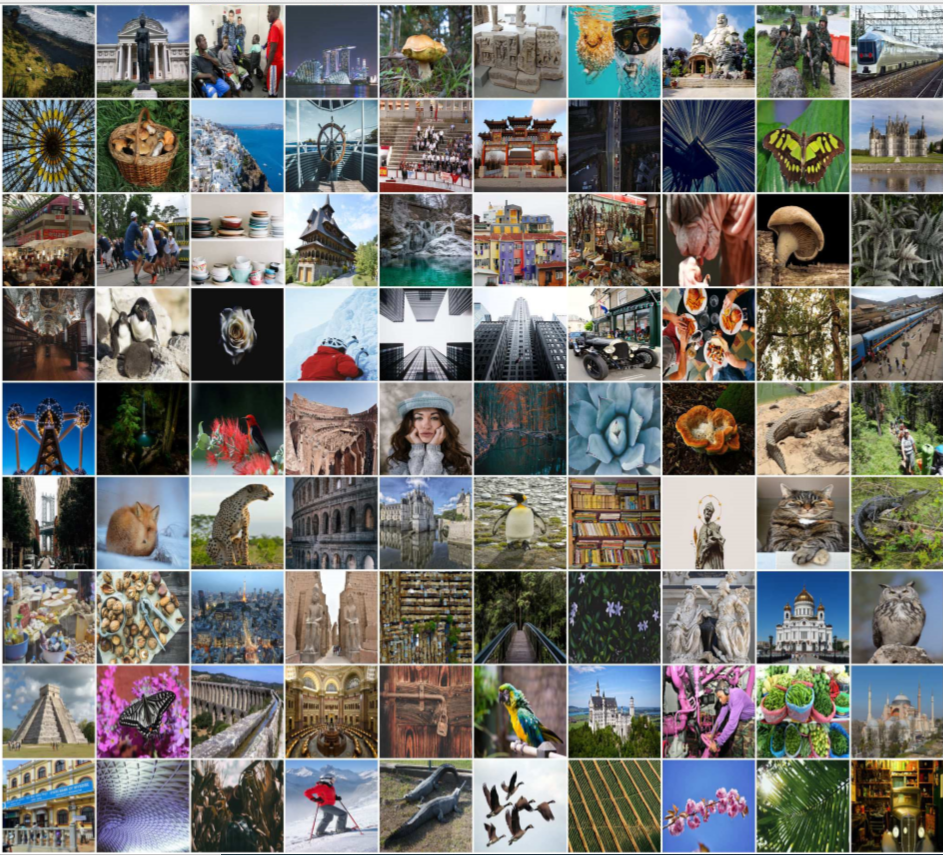
\includegraphics[width=0.85\textwidth]{div2k.png}
\caption{DIV2K validation set examples.
}
\label{fig:div2k}
\end{figure}
\end{center}

In our super resolution applications we used as training set the images provided by the DIV2K (\emph{DIVerse 2K resolution high quality images}) dataset~\cite{Agustsson_2017_CVPR_Workshops}.
This dataset was appositely created for the 2017 NTIRE challenge (\emph{New Trends in Image Restoration and Enhancement}).
The NTIRE challenge is an international competition which aims to monitoring the state-of-art in digital image processing and image analysis and it takes place at the CVPR (\emph{Computer Vision and Pattern Recognition}) conference every year.
One of the most important monitored task is the super resolution research progress.
Thus, every year, many research groups propose new super resolution models, mostly based on neural network models, to improve the state-of-art results on this research field.
The challenge is won by the model which performs the higher PSNR value over a validation set extracted on the DIV2K dataset.
For these reason the DIV2K dataset is considered as a standard for super resolution applications.

The dataset contains 800 high-resolution images as training set and their corresponding low-resolution ones, obtained by different down-sampling methods and different scale factors (2, 3, and 4).
A second set of 100 high-resolution images makes the test set on which the model can evaluate its accuracy: also this second set of images have their low-resolution counterpart.
Finally, a third group of 100 images constitutes the validation set, i.e they are blinded images without their corresponding high resolution counterpart, and they are used to evaluate the results of the models in race.

All the 1000 images are 2K resolution, i.e width and height dimensions must have at least 2K pixels.
The images are collected paying particular attention to the quality, diversity of sources (web sites and cameras) and contents.
The DIV2K images, in fact, collect a large diversity of contents, ranging from people, handmade objects and environments (cities, villages) to natural sceneries (including underwater and dim light conditions) and flora and fauna.
In each image we can find more or less complex shapes, geometries and also some words.
We would stress that no one bio-medical image is contented in the dataset since it is very difficult obtain high quality images of this kind (let alone the problems about copyrights and releases).

In our SR applications we used pre-trained\footnote{
  The developed models were not re-trained due to limited time and low computational architectures available.
} neural network models on the DIV2K and we tested their performances over NMR (Nuclear Magnetic Resonance) images.
The models have never seen this kind of images but during the training they learned a large quantity of shapes that can be \quotes{found} also in bio-medical images.
The bio-medical images were provided by the collaboration with the MRPM group of the Physics Department of the University of Bologna and the Bellaria hospital of Bologna.
We thank the volunteers who perform the NMR acquisitions and shared their data.


\end{document}


\documentclass{standalone}

\begin{document}

\section[Segmentation]{Image Segmentation}\label{segmentation:unet}

\begin{center}
\begin{figure}[htbp]
\centering
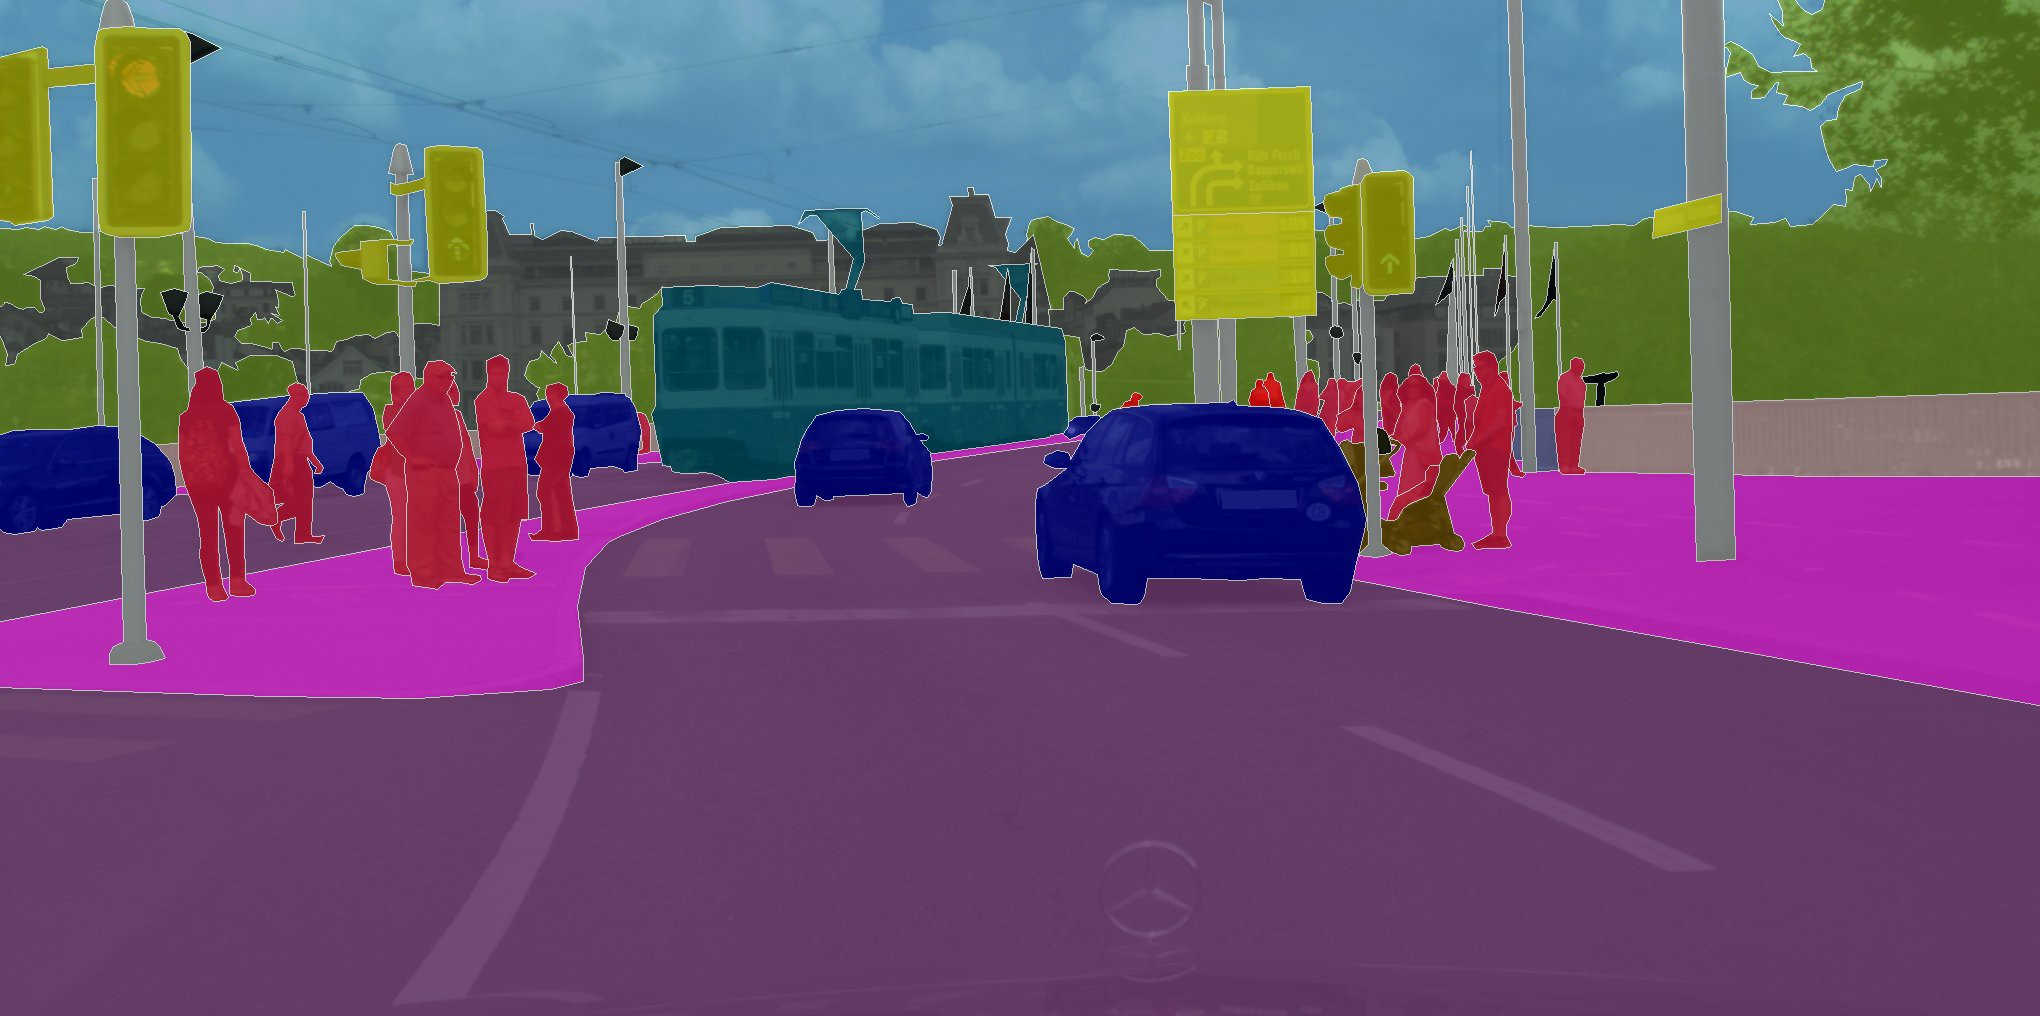
\includegraphics[width=0.85\textwidth]{segmentation.jpg}
\label{fig:segmentation}
\end{figure}
\end{center}

In the previous section we have discussed about the object classification and object detection problems (ref.~\ref{obj_detection:obj}).
Now we want to go deeper on this topic and extract the exact pixels which belong to an object into a given image.
This kind of problem is called Image Segmentation, i.e give a label to each pixel of the input image.

Image segmentation is a typical task in many research fields and could be used for different purposes.
information about pixel-wise position of objects inside an image could be used for extract object shapes from the image or to simplify and/or change the representation of an image into something more meaningful and easier to understand.
This is an hot topic especially for self-driving car applications in which we have to find the exact shapes of object to better estimate their perspective position.
Moreover, all these applications require fast algorithm as much as possible closed to real-time.

This kind of task can be performed using a pipeline of image processing functions or by training a neural network model.
In the first case we have to stack a series of function to process the input image: it has to filters and extracts the useful information about the searched object but most of all it has to be as most general as possible to face on the common heterogeneity of samples.
In the second case we leave to the neural network model parameters the searching of optimal combination of function but we have to provide a supervised input pattern, i.e a combination of input and annotated pixel-wise mask of each image.
The image annotation is one of the most hardest and boring step of image segmentation and for these reasons is very hard to find public dataset usable.

In this chapter we introduce a particular neural network model commonly used in image segmentation problems and we will describe its characteristics and performances.
We applied this model to a novel dataset of CT images.
The dataset annotation was performed by a custom semi-supervised pipeline of image processing and the neural network model was trained and tested on this dataset.
The original data are taken from \href{}{here} and the corresponding annotations are released on \href{}{here}.

\end{document}

\documentclass{standalone}

\begin{document}

\subsection[U-Net model]{U-Net model}\label{segmentation:Unet}

U-Net neural network model is one of the state-of-art model in image segmentation.
It was firstly developed for biomedical image segmentation but it shew its efficiency also in different application tasks and different research topics.
Its backbone is intrinsically a \quotes{common} CNN but the structure can be divided into two macro paths.
The first path of the model is a contraction path (or \emph{encoder}) while the second path is an expansion path (or \emph{decoder}).
The first set of layers in the model, in fact, are a sequence of convolutional and pooling layers which aim to extract features and reduce the dimensionality of the input in the same way as an encoder convert a signal to a smaller range of values.
The extracted features are then processed by the decoder, i.e a second set of convolutional and up-sampling layers, to reconstruct the feature map size and the segmentation mask.
An illustrative representation of the model structure is provided in Fig.~\ref{fig:unet}.

\begin{center}
\begin{figure}[htbp]
\centering
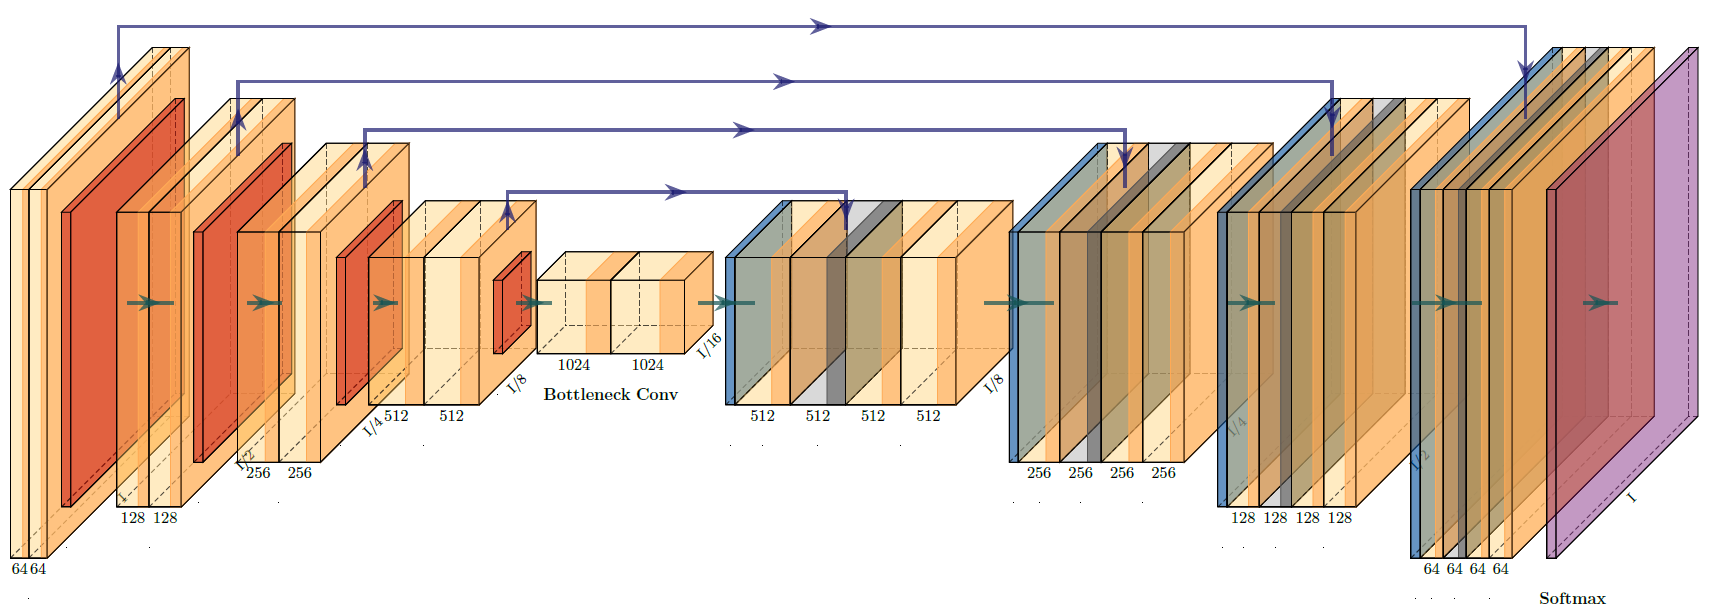
\includegraphics[width=0.85\textwidth]{unet.png}
\caption{U-Net model scheme.
The first part of the structure represents the encoder while the tail of the model is the decoder part.
The model name is given by the numerous shortcut connections which link the encoder layers to the decoder ones: if we contract the long-range connections the global structure acquire a U form.
The figure was generated using the \href{https://github.com/HarisIqbal88/PlotNeuralNet}{PlotNeuralNet} package of H. Iqbal.
}
\label{fig:unet}
\end{figure}
\end{center}

We have already discussed about the functionality of each layers in the previous sections and also in this kind of model a key role was performed by the shortcut connections.
The decoding path tends to lose some of the higher level features the encoder learned: using shortcut connections the output of the encoding layers are passed directly to the decoding layers so that all the important pieces of information can be preserved.

In the previous sections we have also described the common loss functions used to train Neural Network models.
Considering the \quotes{simple} segmentation of an object from its background, the ground truth mask, i.e the \quotes{label} of the input image, would be a binary matrix.
In these cases a valid loss function (also used in our applications) could be the \emph{binary cross-entropy} (ref. \ref{NN:cost}).

\begin{center}
\begin{figure}[htbp]
\centering
\def\svgwidth{0.85\textwidth}
\input{./img/iou_example.pdf_tex}
\caption{IoU score example.
The IoU score is computed as the area intersection of the two boxes over their union.
Starting from the left we can see an increment of the overlap between the two boxes related to an increment in their IoU scores.
}
\label{fig:iou_example}
\end{figure}
\end{center}

A word of caution must be spent about the metrics to evaluate the performances of our model.
Standard metrics, as the \emph{accuracy}\footnote{
  The accuracy measures the number of true positives + false negatives outputs on the total number of predictions.
}, are not good measures to face on the segmentation problem.
If we want to identify and segment an object into an image we can reasonably assume that the number of pixels concerning the object would be very few against the number of pixels related to the background.
Thus the told above binary mask would be a matrix with a large amount of zeros and only few ones.
In this case the standard metric functions have to consider an unbalanced number of samples: if the model outputs a matrix of all zeros the accuracy of it will be high despite the informative values are only the few pixel equals to one.
A possible solution to overcome this problem is given by the \emph{mean IoU score} which measures the average IoU between the output mask and the binary ground truth:

$$
\mbox{IoU} = \frac{\mbox{Area of Overlap}}{\mbox{Area of Union}}
$$

The efficiency and meaning of this score can be visible in Fig.~\ref{fig:iou_example}.

\end{document}

\documentclass{standalone}

\begin{document}

\subsection[CT Dataset]{Femur CT Dataset}\label{segmentation:ct}

The training of a deep Neural Network model as the U-Net one requires a large set of image with corresponding labels.
We developed some experiments on automatic segmentation into a (work in progress) project commissioned by the Rizzoli Hospital of Bologna.
The main task was to develop an automatic pipeline of image processing to extract the 3D femur structure starting from CT (\emph{Computer Tomography}) images.
In particular the crucial point was to improve the identification and segmentation of the femoral head, trying to discriminate this part of the bone from the articular cartilage and moreover from the acetabular fossa.
The project was developed in collaboration with the Engineering group of the professor Viceconti and it aims to study the osteoporosis syndrome and its consequences.

In this work no data were provided by the Rizzoli Hospital and it is hard to find annotated biomedical images (public) on-line, especially about the region of our interest.
We found only few samples of femur CT images (4 patients) and these they are certainly not enough for an accurate training of the model.
To overcome this issue we applied a huge data augmentation pre-processing: each image was randomly rotated, shifted and mirrored.
Moreover we had to face on the problem of data annotation which is always a difficult and time expensive task: we did not have accurate medical annotation so we had to perform them by ourself.

\begin{figure}[htbp]
\centering
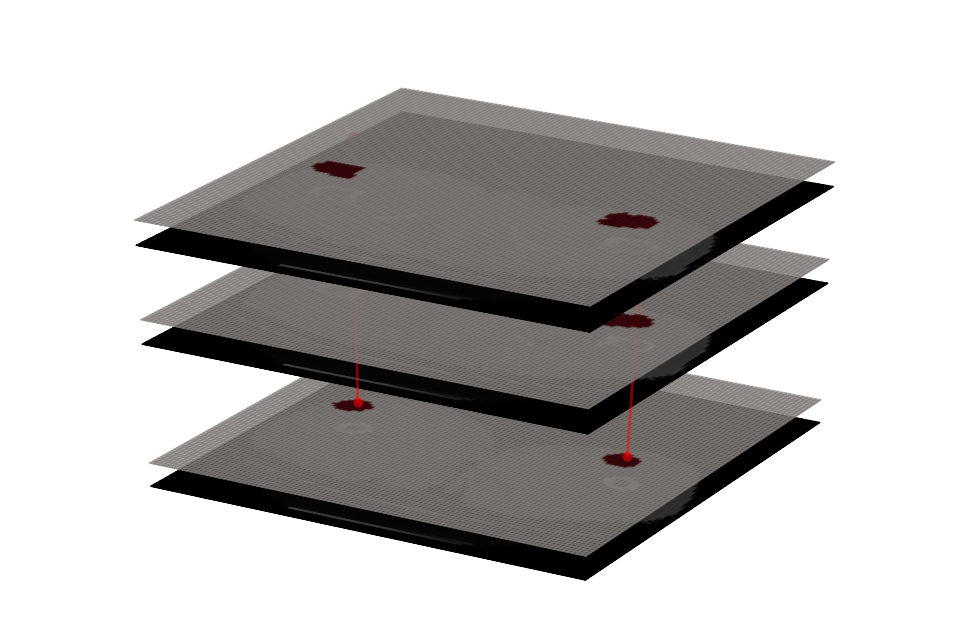
\includegraphics[width=0.85\textwidth]{3D_tool.png}
\caption{Naive segmentation pipeline applied to a series of CT slices.
The thresholding algorithm combined with morphological operations allow to obtained a naive segmentation of the femur bone.
The centroid of the segmented connected components is used to filter the false positive results.
This pipeline was used to simplify the annotation procedure of the CT dataset.
}
\label{fig:3D_tool}
\end{figure}

The annotation was performed using a semi-automatic approach.
We developed a custom image processing pipeline and we applied a combination of thresholding and morphological operators to extract as better as possible the bone structure from each CT frame.
The thresholding operation produced many false positive into the single image which had to be filtered.
To this purpose we could (reasonably) assume that the femur position does not change between two following images.
Thus, once the multiple pixel connected components were identified we filtered them according to their relative position into the image: each group of pixels obtained by the thresholding has its own centroid which remain quite the same also into the next slice (ref. Fig.\ref{fig:3D_tool}).
An interpolation of these components was performed to select only the femur components.
This method worked quite good when we considered the slices far from the femur head: when the acetabular fossa became very close the femur head the two components were not divided.
An example of this kind of issues is shown in Fig.~\ref{fig:seg_tool}.

\begin{figure}[htbp]
\centering
\def\svgwidth{0.85\textwidth}
\input{./img/segmentation_tool.pdf_tex}
\caption{Example of automatic segmentation using custom image processing pipeline.
Starting from the bottom of femur bone the detection seems good but when the method starts to fail the failure is propagated to the next slices.
The method is too naive to perform a good segmentation on the full set of slices.
However, it can be useful to reduce the quantity of slices to annotate manually.
}
\label{fig:seg_tool}
\end{figure}

This naive approach for the image processing could not solve the full segmentation task but it can be considered as a good preliminary tool to produce annotated image.
With this approach we reduced the amount of required annotations by more than 50\%.
The other part of the images were manually annotated.
The manual annotation was performed without any medical background and thus we can not ensure the goodness of our results.
This work only aims to proof the possibility of using deep learning techniques to face on segmentation problems.

Following this approach we were able to annotate 104 CT images randomly sampled from the 4 patient slices.
In particular we extracted 40 slices from a single patient and 96 from the remaining three.
In this way we could use the 96 images as training set (applying the told above image augmentation) and the 40 remaining slices as test set.
We chose to use a single patient slices as test set because with the output generated by the U-Net model we want to reconstruct the (approximated) 3D structure of the femur bone.


\end{document}


\documentclass{standalone}

\begin{document}

\section[rFBP]{Replicated Focusing Belief Propagation}\label{rfbp:rfbp}

Up now we have implicitly talked about Neural Network models based on the standard updating rule of back-propagation.
Other learning rule for weight updates were proposed and the choice of the best one it is still an open-problem.
The final purpose is to obtain a feasible learning rule ables to model the biological learning of the human brain.

The learning problem could be faced through statistical mechanic models joined with the so-called Large Deviation Theory.
In general, the learning problem can be split in two sub-parts: the classification problem and the generalization one.
The first aims to completely store a pattern sample, i.e a prior known ensemble of input-output associations (\emph{perfect learning}).
The second one corresponds to compute a discriminant function based on a set of features of the input which guarantees a unique association of a pattern.

From a statistical point-of-view many Neural Network models have been proposed and the most promising seems to be spin-glass models based.
Starting from a balanced distribution of the system, generally based on Boltzmann distribution, and under proper conditions, we can prove that the classification problem becomes a NP-complete computational problem.
A wide range of heuristic solutions to that type of problems were proposed.

In this section we show one of these algorithms developed by Zecchina et al.~\cite{BaldassiE7655} and called \emph{Replicated Focusing Belief Propagation} (rFBP).
The theoretical background of the algorithm is beyond the scope of this thesis so we focus on its numerical implementation and optimization.

Moreover, despite their proved theoretical efficiency, the applications on real data are still few.
Thus, we show the application of the optimized version of the rFBP algorithm on a Genome Wide Association (GWA) dataset provided by the European \href{https://www.compare-europe.eu/}{COMPARE project}.
This work was also presented on the 2019 CCS-Italy (Conference of Complex System)~\cite{DallOlioCCS19}.

\end{document}

\documentclass{standalone}

\begin{document}


\subsection[Algorithm Optimization]{Algorithm Optimization}\label{rfbp:rFBP}

The rFBP algorithm is a learning algorithm developed to justify the learning process of a binary neural network framework.
The model is based on a spin-glass distribution of neurons put on a fully connected neural network architecture.
In this way each neuron is identified by a spin and so only binary weights (-1 and 1) can be assumed by each entry.
The learning rule which controls the weight updates is given by the Belief Propagation method.

A first implementation of the algorithm was proposed in the original paper~\cite{BaldassiE7655} jointly with an open-source Github repository.
The original version of the code was written in Julia language and despite it is a quite efficient implementation the Julia programming language stays on difficult and far from many users.
To broaden the scope and use of the method, a C++ implementation was developed with a joint \emph{Cython} wrap for Python users.
The C++ language guarantees better computational performances against the Julia implementation and the Python version enlarge its usability.
This implementation is optimized for parallel computing and is endowed with a custom C++ library called \emph{Scorer} (see Appendix D for further details), which is able to compute a large number of statistical measurements based on a hierarchical graph scheme.
With this optimized implementation we try to encourage researchers to approach these alternative algorithms and to use them more frequently on real context.

As the Julia implementation also the C++ one provides the entire rFBP framework in a single library callable via a command line interface.
The library widely uses template syntaxes to perform dynamic specialization of the methods between two magnetization versions of the algorithm.
The main object categories needed by the algorithm are wrapped in handy C++ objects easy to use also from the Python interface.
A further optimization is given by the reduction of the number of available functions: in the original implementation a large amount of small functions are used to perform a single complex computation step, enlarging the amount of call stack; in the C++ implementation the main functions are re-written with the minimizing the call stack to ease the vectorization of the code.

The full rFBP library is released under MIT license and it is open-source on Github~\cite{ReplicatedFocusingBeliefPropagation}.
The on-line repository provides also a full list of installation instructions which could be performed via \emph{CMake} or \emph{Makefile}.
The continuous integration of the project is guaranteed in every operative system using \emph{Travis CI} and \emph{Appveyor CI} which test more than 15 different C++ compilers and environments.

The Python wrap guarantees also a good integration with the other common Machine Learning tools provided by \emph{scikit-learn} Python package; in this way we can use the rFBP algorithm as equivalent alternative also in other pipelines.
Like other Machine Learning algorithm also the rFBP one depends on many parameters, i.e its hyper-parameters, which has to be tuned according to the given problem.
The Python wrap of the library was written according to \emph{scikit-optimize} Python package to allow an easy hyper-parameters optimization using the already implemented classical methods.


\begin{figure}[htbp]
\centering
\def\svgwidth{0.85\textwidth}
\input{./img/rfbp_magp_timing.pdf_tex}
\caption{Comparison of time performances between the original Julia implementation and our Cython one of the rFBP algorithm varying the input dimension sizes (number of samples, $M$, and number of variables, $N$).
For each input configuration 100 runs of both algorithm were performed and the results were normalized by the Julia implementation.
In these cases we fixed the magnetization to \textbf{MagP64}.
}
\label{fig:rfbp_magp}
\end{figure}

\begin{figure}[htbp]
\centering
\def\svgwidth{0.85\textwidth}
\input{./img/rfbp_magt_timing.pdf_tex}
\caption{Comparison of time performances between the original Julia implementation and our Cython one of the rFBP algorithm varying the input dimension sizes (number of samples, $M$, and number of variables, $N$).
For each input configuration 100 runs of both algorithm were performed and the results were normalized by the Julia implementation.
In these cases we fixed the magnetization to \textbf{MagT64}.
}
\label{fig:rfbp_magt}
\end{figure}
%30 (N,M) con N in 1001-5001 con 1000, M=101-351 con 50 ognuna 100 magT

We firstly test the computational efficiency of our implementation against the original Julia one.
The tests were performed comparing our \emph{Cython} version of the code (and thus with a slight overhead given by the Python interpreter) and the Julia implementation as reference.
Varying the dimension sizes (number of samples, $M$, and number of variables, $N$) we tested the time efficiency over 100 runs of both the algorithms.
We divided our simulation according to the two possible type of magnetizations (MagP64 and MagT64 as described by the original implementation available \href{https://github.com/carlobaldassi/BinaryCommitteeMachineFBP.jl}{here}) and the obtained results are shown in Fig.~\ref{fig:rfbp_magp}~\ref{fig:rfbp_magt}, respectively.

As can be seen by the two simulations our implementation always overcome the time performances of the original one, taken as reference in the plot.
However, we can not guarantee a perfect parallel execution of our version: also with multi-threading support the scalability of our implementation does not follow a linear trend with the number of available cores.
In our simulation, in fact, we used 32 cores against the single thread execution of the Julia implementation but we gained only a 4x and 2x of speedup for MagT64 and MagP64, respectively.
The network training is a sequential process by definition and thus it is hard to obtain a relevant speedup using a parallel implementation.
In this case it is probably jointed to a not perfect parallelization strategy chosen which bring to a not efficient scalability of our algorithm version.
However, the many improvements performed to the code allow us to use this algorithm with bigger dataset sizes.

\end{document}

\documentclass{standalone}

\begin{document}


\subsection[Compare dataset]{SNP classification}\label{rfbp:snp}

The few available applications of the rFBP algorithm to real data are amenable to two aspects: I) learning technique; II) algorithm implementation.
The first one is related to the intrinsic definition of the algorithm which is designed to reach a complete memorization of the training dataset; in the other Machine Learning processes we normally want to avoid this kind of results since it could bring to \emph{over-fitting} problems.
The second one is given by the binary values involved in each step of the algorithm which intrinsically limit the possible applications\footnote{
  The Neural Network weights can assume only binary values since they model up/down spins.
  Moreover also the input is required to be a spin configuration and thus binary.
  The common Machine Learning problems involve floating-point values as input pattern.
}.


Classification problems which involved only binary quantities are quite small but the GWA is one of them.
In the GWA we have a series of genome data belonging to different classes as input.
A genome is the ensemble of genes of an organism and each gene is identified by a series of nucleotides with 4 possible values (G, guanine; C, cytosine; A, adenine; T, thymine).
The comparison between a reference (healthy) genome and an infected one highlights the biological mutation related to the understudy disease.
This mutation are the so-called SNPs (Single Nucleotide Polymorphisms).
So we can identify a genome as a sequence of its mutation in relation to a reference genome, i.e a sequence of two possible values given by the on/off of the mutation in each nucleotide.

The COMPARE project aims to develop new methods to avoid the genetic disease transmission.
In this project plays a crucial role the \emph{Source Attribution}, i.e the classification of a given disease based on the list of its mutation.

We tested the rfBP on $210$ Salmonella enterica genome sequences, $4857450\,bp$ (base pairs) long, living inside animals.
Our early goal was to discriminate those bacteria living in pigs (159 samples) with respect to all the others animals (51 samples).

First of all we filter our data removing from each genome a base if it is not mutated in each sample.
In this way we reduce the number of bases to $8189\,bp$.
A graphical representation of these samples is given in Fig.~\ref{fig:SNPsAle}.
The dataset was divided in training and test sets using a stratified cross-validation procedure to guarantee a proportional subdivision of the samples into the two classes.
The algorithm hyper-parameters was tuned on the training set based on the performances obtained using a internal stratified 10-fold cross-validation: in each fold the training was performed by a given sequence of hyper-parameters and the performances evaluated on the corresponding test set; the hyper-parameters configuration which obtains the best performances on the full training set was chosen as best configuration.
The performances evaluation was performed using the custom \emph{Scorer} library.
Considering the unbalanced sample quantities the Matthews Correlation Coefficient (MCC) is chosen as good scorer indicator for the evaluation.

With the tuned hyper-parameters we performed the training of rFBP algorithm on different percentage of the training set: $25\%$, $45\%$, $65\%$ and $85\%$.
In the same way we train also a list of the most common Machine Learning classifiers: single perceptron with floating-point weights (Perc); standard Neural Network with gradient descent as updating rule (MLP); support vector machine with linear kernel (lSVM); support vector machine with radial kernel (rSVM); linear discriminant analysis (LDA); decision tree (DT); random forest (RF); k-nearest neighbors with 2-clusters (kNN); Guassian process (GP); diag-quadratic discriminant analysis (GNB); Bernoulli naive bayes (BNB); AdaBoost (AdaB).
For each training percentage we perform the optimization of the hyper-parameters of each classifier with the same number of optimization steps.
In Fig.~\ref{fig:confronto_bestclassificatoriACC, fig:confronto_best_classificatoriMCC} the accuracies and MCC results are shown, respectively.

From this analysis we can conclude that the rFBP algorithm shows comparable performances with the other classifiers.
These performances globally grow with the training set size but only the rFBP is able to reach a \quotes{perfect learning} configuration, i.e accuracy of 100\% and MCC=1.
We have also noticed that the rFBP classifier and the GNB are the only two algorithms which qualitatively does not show performances saturation on their training.

A second analysis was performed on the data distribution using a multiple $\chi^2$-test.
Starting from the whole set of genomes we can compute the contingency-matrix of the two classes\footnote{
  The contingency-matrix displays the (multivariate) frequency distribution of the variables.
  Each row will count the number of hosts with/without the SNPs.
  Each column will identify a class.
}.
The $\chi^2$-test was performed on the full set of $8189\,bp$ and so the extracted \emph{p-values} were corrected according multiple-tests.
Using the \v{S}id\'ak~\cite{Sidak1967} correction method and by the definition of significant threshold of $0.05$ we found $1103$ significant bases.
An analogous $\chi^2$-test was performed on the rFBP weights to identify a putative

% MISS

\end{document}

\documentclass{standalone}

\begin{document}

\subsection[Results]{Results}\label{rfbp:snp_result}

\begin{figure}[htbp]
\centering
\def\svgwidth{\textwidth}
\input{./img/Ale_ACC_confrontoNicoPhD.pdf_tex}
\caption{Accuracy score obtained on the validation set varying the training set size.
We compared the trends of the whole set of classification algorithms used.
}
\label{fig:confronto_bestclassificatoriACC}
\end{figure}


\begin{figure}[htbp]
\centering
\def\svgwidth{\textwidth}
\input{./img/Ale_MCC_confrontoNicoPhD.pdf_tex}
\caption{Matthews Correlation Coefficient (MCC) score obtained on the validation set varying the training set size.
We compared the trends of the whole set of classification algorithms used.
}
\label{fig:confronto_bestclassificatoriMCC}
\end{figure}

With the tuned hyper-parameters we performed the training of rFBP algorithm on different percentages of the training set: $25\%$, $45\%$, $65\%$ and $85\%$.
In the same way we trained also a list of the most common Machine Learning classifiers: simple Perceptron with floating-point weights (Perc); standard Neural Network with gradient descent as updating rule (MLP); support vector machine with linear kernel (lSVM); support vector machine with radial kernel (rSVM); linear discriminant analysis (LDA); decision tree (DT); random forest (RF); k-nearest neighbors with 2-clusters (kNN); Guassian process (GP); diag-quadratic discriminant analysis (GNB); Bernoulli naive bayes (BNB); AdaBoost (AdaB).
For each training percentage we performed the optimization of the hyper-parameters of each classifier with the same number of optimization steps.
In Fig.~\ref{fig:confronto_bestclassificatoriACC}~\ref{fig:confronto_bestclassificatoriMCC} the accuracies and MCC results are shown, respectively.

From this analysis we can conclude that the rFBP algorithm shows comparable performances with the other classifiers.
These performances globally grow with the training set size, but only the rFBP was able to reach a \quotes{perfect learning} configuration, i.e accuracy of 100\% and MCC=1.
We have also noticed that the rFBP classifier and the GNB were the only two algorithms which qualitatively does not show performance saturation on their training.

A second analysis was performed on the data distribution using a multiple $\chi^2$-test.
Starting from the whole set of genomes we can compute the contingency-matrix of the two classes\footnote{
  The contingency-matrix displays the (multivariate) frequency distribution of variables.
  Each row counts the number of hosts with/without the SNPs.
  Each column identifies a class.
}.
The $\chi^2$-test was performed on the full set of $8189\,bp$ and so the extracted \emph{p-values} were corrected according multiple-tests.
Using the \v{S}id\'ak~\cite{Sidak1967} correction method and by the definition of significant threshold of $0.05$ we found $1103$ significant bases.
An analogous $\chi^2$-test was performed on the rFBP weights to identify a putative correlation between a set of weights and mutated bases.
This second $\chi^2$-test was performed only on the simulation which involved the 85\% of data as training set because it was the case in which the rFBP algorithm shows the better performances than the other classifiers.
We firstly defined a base as significant if its corresponding p-value was less or equal than 0.05: in this way we could associate to each base a numerical weight of 0 if it was not significant an $+1$ or $-1$ if it was, where $+1$ identified the pig class and $-1$ the other one.
The set of weights defined following these instruction could be associated to the \quotes{ideal set}.
In this way we could ensure that if the corresponding rFBP weights were equal to $+1$ in all the significant positions (and thus in all the significant bases) for the pig class, the model output would be $+1$ and $-1$ in the opposite case.
This mechanism follows the Simple Perceptron algorithm scheme (ref. \ref{NN:perceptron}) in which each weight is associated to a given entry of the input samples.
The rFBP algorithm follows the same rules with an activation function given by the Heaviside $\Theta$ and it changes only the updating rule.
Moreover, following this method we could ensure that only the $1103$ significant bases extracted were associated to a not null weight.

We took into account the 10 weights set extracted by the 10-Fold cross validation performed to extract the previous results.
From these 10 sets we extracted the representative one using a simple average of their values: each weight entry was computed as the mean of the 10 weight realizations.
In this way each weight entry was converted to a floating point number and we can easily extract the set of weights perfectly equal to $\pm1$.
From our analyses $5201$ weights were consistently equal to $\pm1$ in all the simulations, i.e the algorithm assigned to $5201$ weights always the same value.
In this way we could consider these weight entries as the significant positions identified by the rFBP algorithm.

These rFBP significant weight set could be compared to the $\chi^2$ ideal set.
From this comparison we noticed a good agreement between the two sets: the major part of the significant bases for the $\chi^2$ multiple test could be found also in the significant weights identified by the 10 realizations of the rFBP algorithm.
In particular, we found that $838/841$ bases were significant for both the methods.
The rFBP algorithm correctly identified $838/848$ significant bases related to the $-1$ class and only $3/255$ bases related to the $+1$ class.

In conclusion, we could prove that the rFBP algorithm is able to identify the major part of the significant polymorphisms in the training set.
However, the use of the only training set to extract the significant weights certainly penalized the rFBP algorithm and a second simulation (without prediction purposes) was performed considering the full set of data, i.e 10 realizations without cross-validation.
In this second case the rFBP significant weights correctly identified $702/1103$ where $696/848$ were related to the $-1$ class and $6/255$ to the $+1$ class.
In both cases we could conclude that the dataset did not contain enough information for the $+1$ class identification for the rFBP algorithm.

Following the above results, a final training was performed using only the significant bases identified by the rFBP algorithm and only the significant bases extracted by the $\chi^2$ multiple test, using the full set of available classifiers.
We noticed how the performances of all the classifiers are significantly better using the bases extracted by the rFBP algorithm (always over the 87\% of accuracy) than the results obtained considering the $\chi^2$ significant bases (only few classifier were able to obtain more than 85\% of accuracy).

We conclude that our results highlight the efficiency of the rFBP algorithm for genome analyses and SNPs classification problems.
Moreover we could propose also the rFBP algorithm as a valid feature selection alternative to classical statistical tests.
These results also encourage us to further investigate about the biological meaning of the significant bases identified.

\end{document}


\end{document}
